%% Mẫu luận án tiến sĩ (thạc sĩ) theo style vietkey.luanan.1.2.cls - Version 1.2
%% (c) Dang Minh Tuan, Vietkey Group. 
%% Tel: +84-98-868-6636, Email: tuanvietkey@gmail.com.
%%
%% History:
%% - version 1.2 (2017/08/11)
%% - Created on 2016/08/16.

\documentclass[fontsize=13pt,oneside,a4paper,openany]{vietkey.luanan.1.2}

\usepackage[backend=bibtex,bibstyle=luanan,sorting=nyvt,block=none,defernumbers=true,babel=other]{biblatex} %tham số firstinits=true để viết tắt, defernumbers để số thứ tự liền mạch.



\addbibresource{bibdmt.bib} %%% dữ liệu về tài liệu tham khảo.
\begin{document} 

\begin{titlepage}		
	\begin{tikzpicture}[remember picture, overlay]
	\draw[line width = 2pt] ($(current page.north west) + (1.3in,-1.1in)$) rectangle ($(current page.south east) + (-0.7in,1.1in)$);
	\end{tikzpicture}
	%\vspace*{-1.15cm}
	\vspace*{-0.7cm}
	\begin{center}
		\begin{minipage}{0.45\textwidth}
			\begin{flushleft} 
				BỘ GIÁO DỤC VÀ ĐÀO TẠO
			\end{flushleft}
		\end{minipage}
		\begin{minipage}{0.45\textwidth}
			\begin{flushright} 
				BỘ QUỐC PHÒNG
			\end{flushright}
		\end{minipage}
		\\[0.03cm]
		% Upper part of the page
		{\bfseries VIỆN KHOA HỌC VÀ CÔNG NGHỆ QUÂN SỰ }\\[4.4cm]
		
		{\large \bfseries Đặng Minh Thảo}\\[2.7cm]
		
		
		{ \bfseries \large NGHIÊN CỨU XÂY DỰNG MỘT SỐ DẠNG\\[0.0cm]LƯỢC ĐỒ MỚI CHO CHỮ KÝ SỐ TẬP THỂ }\\[2.4cm]
		{\bfseries LUẬN ÁN TIẾN SĨ TOÁN HỌC }\\[8cm]
		
		%\vfill
		
		% Bottom of the page
		{\bfseries Hà Nội -- 2027}		
	\end{center}
\end{titlepage}
\begin{titlepage}		
	\begin{tikzpicture}[remember picture, overlay]
	\draw[line width = 2pt] ($(current page.north west) + (1.3in,-1.1in)$) rectangle ($(current page.south east) + (-0.7in,1.1in)$);
	\end{tikzpicture}
	\vspace*{-0.7cm}
	\begin{center}
		\begin{minipage}{0.45\textwidth}
			\begin{flushleft} 
				BỘ GIÁO DỤC VÀ ĐÀO TẠO
			\end{flushleft}
		\end{minipage}
		\begin{minipage}{0.45\textwidth}
			\begin{flushright} 
				BỘ QUỐC PHÒNG
			\end{flushright}
		\end{minipage}
		\\[0.04cm]
		% Upper part of the page
		{\bfseries VIỆN KHOA HỌC VÀ CÔNG NGHỆ QUÂN SỰ }\\[4.1cm]
		
		{\large \bfseries Đặng Minh Thảo}\\[2.1cm]
		
		
		{ \bfseries \large NGHIÊN CỨU XÂY DỰNG MỘT SỐ DẠNG\\[0.0cm] LƯỢC ĐỒ MỚI CHO CHỮ KÝ SỐ TẬP THỂ }\\[0.7cm]
	\end{center}
	%\scalebox{.95}[1.0]{\large Chuyên ngành: Cơ sở toán học cho tin học}
	\hspace*{2.7cm}{\large Chuyên ngành: Cơ sở toán học cho tin học}\\[0.0cm]
	\hspace*{2.7cm}{\large Mã số: 62 46 01 10}\\[0.0cm]
	\begin{center}
		{\bfseries LUẬN ÁN TIẾN SĨ TOÁN HỌC }\\[0.7cm]
	\end{center}
	\hspace*{6.7cm}{\bfseries NGƯỜI HƯỚNG DẪN KHOA HỌC:}\\[0.1cm]
	\hspace*{7.9cm}{ 1. PGS. TS Nguyễn Văn A}\\[0.0cm]
	\hspace*{7.9cm}{ 2. PGS. TS Đặng Đình B}\\[3.6cm]
	\begin{center}	
		%\vfill
		
		% Bottom of the page
		{\bfseries Hà Nội -- 2027}
	\end{center}		
\end{titlepage}  	%%% có thể thay đổi

\VKnumRoman				%%% đánh số bằng chữ cái i, ii...

\textit{\textbf{Xin chào}}

\[{\sqrt{\frac{-1+{\sqrt{1+{\frac{1}{4}}(x^{2}-2^{n})^{2}}}}{1+{\sqrt{1+{\frac{1}{4}}(x^{2}-2^{n})^{2}}}}}={\frac{1-2^{n}}{1+2^{n}}}}\]

\begin{itemize}
	\item 123
	\item 345
	\item 456
\end{itemize}

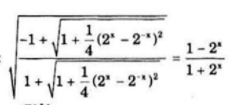
\includegraphics[scale=0.5]{image3_gLrwE}

\[y={\frac{3x^{3}+3x}{x}}\]


\includegraphics[scale=1]{RBqEh}


\includegraphics[scale=1]{geh6V}

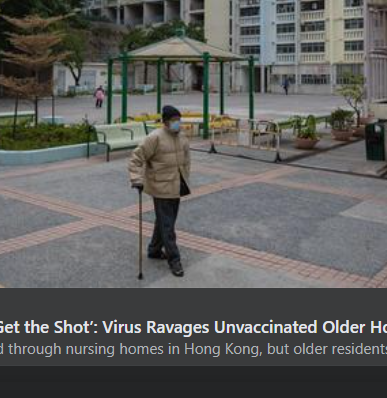
\includegraphics[scale=1]{oGA08}

\subsection{12312312}


\chapter*{LỜI CAM ĐOAN}
%\addcontentsline{toc}{section}{{\bf LỜI CAM ĐOAN}\rm}
%\thispagestyle{empty}
%
%\markboth{{\it Lời nói đầu}}{{\it Lời nói đầu}}

Tôi xin cam đoan các kết quả trình bày trong luận án là công trình nghiên cứu của tôi dưới sự hướng dẫn của các cán bộ hướng dẫn. Các số liệu, các kết quả trình bày trong luận án hoàn toàn trung thực và chưa được công bố trong các công trình trước đây. Các dữ liệu tham khảo được trích dẫn đầy đủ và chính xác nhất.

\hfill \textit{Hà Nội, ngày 10 tháng 06 năm 2027}
\newline
\newline
\newline

\hfill {\bf Đặng Minh Thảo}\hspace{1.5cm}
\newline
\begin{center}
{\color{red}(Xem hướng dẫn sử dụng \LaTeX\ tại Chương 2 trang \pageref{chchukytapthedathanhphan}).}
\end{center}	%%% có thể thay đổi

\chapter*{LỜI CẢM ƠN}
\addcontentsline{toc}{section}{{\bf LỜI CẢM ƠN}\rm}
%\thispagestyle{empty}
%
%\markboth{{\it Lời nói đầu}}{{\it Lời nói đầu}}

\(T=\frac{1}{2}\left(T_{1}+T_{2}\right)=\frac{1}{2}\;\left(2\pi\sqrt{\frac{l_{1}}{g}}+2\pi\sqrt{\frac{l_{2}}{g}}\right)=1,5s\)

Trong quá trình nghiên cứu và hoàn thành Luận án, Nghiên cứu sinh đã nhận được sự định hướng, giúp đỡ, các ý kiến đóng góp quý báu và những lời động viên của các nhà khoa học, các thầy cô giáo, đồng nghiệp và gia đình.

Trước hết, Nghiên cứu sinh xin bày tỏ lời cảm ơn tới các thày PGS.TS Nguyễn Văn A, PGS.TS Đặng Đình B đã tận tình hướng dẫn và giúp đỡ trong quá trình nghiên cứu. 

Cho phép Nghiên cứu sinh chân thành cảm ơn các thày cô giáo, các nhà khoa học của Viện Khoa học và Công nghệ quân sự, Viện Công nghệ thông tin, Viện Toán học,\ldots  đã có các góp ý quý báu cho Nghiên cứu sinh trong quá trình thực hiện Luận án này một lần nữa

Nghiên cứu sinh chân thành cảm ơn Ban Giám đốc, Phòng Đào tạo, Viện Khoa học và Công nghệ quân sự đã tạo điều kiện thuận lợi để Nghiên cứu sinh hoàn thành nhiệm vụ nghiên cứu. 

Cuối cùng Nghiên cứu sinh bày tỏ lời cảm ơn tới các đồng nghiệp, gia đình, bạn bè đã luôn động viên, chia sẻ, ủng hộ và giúp đỡ Nghiên cứu sinh vượt qua khó khăn để đạt được những kết quả nghiên cứu trong Luận án này.\\[0.03cm]

\hfill {\bf NCS Đặng Minh Thảo}\hspace{1.3cm}

\[\textstyle\bigsqcup{\sqrt{\ +}}\sqrt{\j_{U}}\to\ {\theta}^{\gamma}\longrightarrow\ {\overset{\prime}{\longrightarrow}}\ {\overset{\mathcal{\rightarrow}}{\mathcal{\prime}}}\]		%%% có thể thay đổi

\VKmucLuc				%%% mục lục

\chapter*{DANH MỤC CÁC KÝ HIỆU, CÁC CHỮ VIẾT TẮT}
%\markboth{{\it Phương pháp đại lượng bất biến}}{{\it Kí hiệu}}
\addcontentsline{toc}{section}{{\bf DANH MỤC CÁC KÝ HIỆU, CÁC CHỮ VIẾT TẮT}}
\begin{center}
\begin{tabular}{ l  l }
$\left\lbrace 0,1\right\rbrace^*$ & Ký hiệu chuỗi bit có độ dài bất kỳ \\
$\left\lbrace 0,1\right\rbrace^\infty$ & Ký hiệu chuỗi bit có độ dài vô tận \\
$\epsilon$ & Hàm nhỏ không đáng kể\\
$\sigma$ & Chữ ký số\\
$\perp$ & Thuật toán không cho ra kết quả\\
$\mathfrak{V}$ & Vector phân công ký tập thể\\
ACMA & Tấn công văn bản được lựa chọn thích ứng\\& (Adaptive Chosen Message Attacks) \\
CDH & Bài toán Deffie-Hellman (Computational Diffie-Hellman)\\
$\det$& Định thức\\
$d$ & Khóa bí mật trong hệ mật ECC\\
DSA & Thuật toán chữ ký số (Digital Signature Algorithm) \\
$e$ & Giá trị băm của hàm băm $e=H(m)$\\
EC & Đường cong Elliptic (Elliptic Curve) \\
ECC & Hệ mật dựa trên đường cong Elliptic (Elliptic Curve Cryptography) \\
ECDH & Thuật toán Elliptic Curve Diffie–Hellman \\
ECDLP & Bài toán logarithm rời rạc (Elliptic Curve Logarithm Problem) \\
ECDSA & Thuật toán chữ ký số dựa trên đường cong elliptic\\& (Elliptic Curve Digital Signature Algorithm)\\
FPGA & Mạch tích hợp cỡ lớn có khả năng lập trình \\& (Field-Programmable Gate Array)\\
$\mathbb {F}$ & Trường hữu hạn\\
$\gcd$ & Ước số chung lớn nhất (Greatest Common Divisor)\\
$H$ & Hàm băm (Hash fuction)\\
\end{tabular}
\end{center}

		%%% có thể thay đổi

\VKdanhMucHinhVe		%%% danh mục hình vẽ 
\VKdanhMucBangBieu		%%% danh mục bảng biểu 
%\VKdanhMucDinhLy
%\VKdanhMucDinhNghia
\VKbatDaudanhSo			%%% bắt đầu đánh số từ 1,2,3...

\chapter*{MỞ ĐẦU}

%\thispagestyle{empty}
%\markboth{{\it Lời nói đầu}}{{\it Lời nói đầu}}

\addcontentsline{toc}{section}{{\bf  MỞ ĐẦU}\rm}

\vspace*{-0.2cm}
\textit{\textbf{Tính cấp thiết của đề tài nghiên cứu:}}

%\cite{S8550}; \cite{S2280}

%\textbf{\textsc{bold small caps}} \textbf{This is bold} and \textsc{this is small caps} and \textsc{\textbf{this is bold small caps.}}
Trong những năm gần đây, các điều kiện về cơ sở hạ tầng và cơ sở pháp lý cho chính phủ điện tử và thương mại điện tử ở Việt Nam đã chín muồi. Cụ thể là theo sách trắng Công nghệ thông tin năm 2014, đến nay Việt Nam đã có gần 33.2 triệu người sử dụng Internet, băng thông Internet quốc tế đã đạt 640 Gbps. Luật giao dịch điện tử đã có hiệu lực từ năm 2005, theo đó, các giao dịch điện tử hoàn toàn có tính pháp lý như những giao dịch thực hiện bằng các văn bản giấy cùng với chữ ký và con dấu truyền thống. Có thể nói, chính phủ điện tử và thương mại điện tử chỉ có thể phát triển được khi và chỉ khi hệ thống chữ ký số, chứng thư số được áp dụng đồng bộ. Bởi vì chính chữ ký số mới có thể bảo đảm tính pháp lý của các giao dịch điện tử.

Về hành lang pháp lý, liên quan đến chữ ký số, chứng thư số, Việt Nam đã có 04 văn bản luật, 10 nghị định, 12 thông tư và 7 quyết định. Sau khi Trung tâm Chứng thực chữ ký số Quốc gia (Root CA) được thành lập vào năm 2008, đến năm 2016 đã có 09 công ty (VDC, Viettel, FPT, Nacencomm, BKAV\ldots) cung cấp chứng thực chữ ký số cho các tổ chức và cá nhân, và có thể cung cấp một số dịch vụ chữ ký số như kê khai thuế qua mạng, hải quan điện tử, ký email, hóa đơn, hợp đồng, đấu thầu điện tử. Tuy nhiên, hiện nay các doanh nghiệp mới chỉ cung cấp các dịch vụ cho chữ ký đơn, khi mỗi người ký số chỉ ký vào một văn bản duy nhất. Mặc dù các điều kiện cơ bản về hạ tầng kỹ thuật và hạ tầng pháp lý đã hội tụ, song chính phủ điện tử và thương mại điện tử ở Việt Nam vẫn chưa phát triển được như mong đợi, một phần là bởi vì các ứng dụng về chứng thư số và chữ ký số vẫn còn chưa được triển khai rộng rãi, các nghiên cứu lý thuyết và thực tiễn áp dụng chữ ký số vẫn còn ở mức rất khiêm tốn.

Chữ ký số tập thể có nhiều ứng dụng trong thực tiễn, ví dụ dùng để kiểm tra đồng loạt nhóm chữ ký số theo lô, xác thực đa yếu tố, hoặc dùng cho các kênh quảng bá: IP Multi-cast, Peer-to-Peer file sharing, grid computing, mobile adhoc networks\ldots

Từ cơ sở trên chúng ta thấy nghiên cứu chữ ký số nói chung và chữ ký số tập thể nói riêng là rất cần thiết, có ý nghĩa to lớn về mặt học thuật cũng như thực tiễn.
%\newpage

\textit{\textbf{Mục tiêu nghiên cứu:}}

Mục tiêu của Luận án là nghiên cứu tổng quan về chữ ký số, chữ ký số tập thể; từ đó phát triển mới một số dạng lược đồ cho chữ ký số tập thể, có thể ứng dụng triển khai trong thực tiễn (chữ ký số tập thể đa thành phần, kết hợp giữa chữ ký số tập thể đa thành phần với chữ ký số mù và với chữ ký số ủy nhiệm\ldots). Chứng minh bằng toán học các lược đồ chữ ký số sẽ xây dựng có tính đúng đắn và độ an toàn đáp ứng được các yêu cầu triển khai thực tiễn.

\textit{\textbf{Nội dung nghiên cứu:}}
\begin{itemize}
	\item Nghiên cứu đề xuất mô hình chữ ký số tập thể đa thành phần.
	\item Đề xuất lược đồ ký tập thể dựa trên hệ mật đường cong elliptic, cặp song tuyến tính, hệ mật dựa trên bài toán logarithm rời rạc.
	\item Nghiên cứu, đề xuất mô hình kết hợp giữa chữ ký số tập thể đa thành phần với chữ ký số ủy nhiệm.
	\item Nghiên cứu, đề xuất mô hình kết hợp giữa chữ ký số tập thể đa thành phần với chữ ký số mù.
\end{itemize}

\textit{\textbf{Đối tượng và phạm vi nghiên cứu:}}

Đối tượng nghiên cứu là lược đồ chữ ký số tập thể, kết hợp với chữ ký số ủy nhiệm, chữ ký số mù trong một số hệ mật mã thông dụng: ElGamal (logarithm rời rạc), elliptic, hệ mật định danh (ID-Based), song tuyến tính.


\textit{\textbf{Phương pháp nghiên cứu:}}

Tham khảo các công trình, bài báo và sách, tài liệu chuyên ngành về lĩnh vực chữ ký số tập thể từ đó đề xuất mô hình mới giải quyết vấn đề còn tồn tại. Sử dụng các lý thuyết về các hệ mật phổ biến để xây dựng các giao thức và lược đồ chữ ký số cho các hệ mật này chứng minh cho mô hình mới phát triển. Sử dụng lý thuyết về độ phức tạp thuật toán để đánh giá độ an toàn và hiệu năng của lược đồ chữ ký số tập thể. Cài đặt thử nghiệm bằng phần mềm và triển khai trên Chip FPGA (Field-Programmable Gate Array), áp dụng vào thực tiễn triễn khai đề tài cấp Nhà nước.

\textit{\textbf{Ý nghĩa khoa học và thực tiễn của luận án:}}

Về mặt lý thuyết, Luận án đã đưa mô hình chữ ký tập thể mới là mô hình tổng quát của nhiều lớp chữ ký số tồn tại trước đây, trên cơ sở mô hình mới này sẽ mở ra hàng loạt hướng nghiên cứu mới kết hợp giữa chữ ký số tập thể đa thành phần với các mô hình chữ ký số khác như chữ ký số mù, chữ ký số ủy nhiệm, chữ ký số ngưỡng, chữ ký số vòng, chữ ký số cấu trúc, đồng thời cũng mở ra nghiên cứu triển khai mô hình này cho các hệ mật khác nhau như hệ mật đường cong elliptic, hệ mật định danh, hệ mật dựa trên nhóm Braid, hệ mật dựa trên nhóm dàn (lattice).

Về mặt thực tiễn, mô hình chữ ký số tập thể đa thành phần do có độ dài chữ ký số không phụ thuộc vào số người ký và số văn bản được phân tách thành các thành phần, vì thế khi số lượng người ký tăng lên thì không gian lưu trữ chữ ký số không bị tăng tuyến tính với số lượng người ký và như vậy sẽ tiết kiệm được rất nhiều không gian lưu trữ và băng thông chuyển tải chữ ký số trên đường truyền. Bên cạnh đó do mô hình chữ ký số tập thể đa thành phần cho phép ký một lần cho tất cả các thành viên và với tất cả các thành phần của văn bản trong một lần nên sẽ tiết kiệm được thời gian tính toán và tài nguyên tính toán để hình thành chữ ký số và xác thực chữ ký số do thời gian và tài nguyên tính toán không bị tăng tuyến tính theo số lượng người ký và số thành phần của văn bản. Chữ ký số tập thể đa thành phần cũng đáp ứng tốt thực tiễn hơn các lược đồ tộn tại, do cho phép số người ký và số phần của văn bản khác nhau.


\textit{\textbf{Bố cục của luận án:}}

Ngoài phần mở đầu và phần kết luận, kiến nghị, Luận án được chia thành 3 chương với bố cục như sau:

%\textbf{Chương \ref{chtongquan}}: \textit{\textsc {Tổng quan về vấn đề nghiên cứu}}.
%
%Chương này tập trung vào trình bày tóm tắt tình hình nghiên cứu về chữ ký số, chữ ký số tập thể, chữ ký số tập thể ủy nhiệm, chữ ký số tập thể mù. 


\textbf{Chương \ref{chtongquan}}: \textsc{Tổng quan về chữ ký số và chữ ký tập thể}.

Chương  \ref{chtongquan} trình bày tình hình nghiên cứu tổng quan về chữ ký số, chữ ký số tập thể, chữ ký số tập thể ủy nhiệm, chữ ký số tập thể mù. Chương này cũng trình bày một số khái niệm và định nghĩa cơ bản về chữ ký số, các loại hình tấn công và phá vỡ lược đồ chữ ký số. Tiếp theo,  chương \ref{chtongquan} đưa ra định nghĩa chữ ký số tập thể và phân loại chữ ký số tập thể.

\textbf{Chương \ref{chchukytapthedathanhphan}}: \textsc{Chữ ký số tập thể đa thành phần}.

Chương này trình bày về kết quả nghiên cứu mới của Luận án đó là mô hình ký số tập thể mới: chữ ký số tập thể đa thành phần. Mô hình mới này cho phép đáp ứng tốt hơn, linh hoạt hơn so với các mô hình ký tập thể hiện có. Mô hình này cũng là mô hình khái quát hóa một số các mô hình trước đây.

Trong chương \ref{chchukytapthedathanhphan}, Luận án cũng định nghĩa chặt chẽ (formal) chữ ký số tập thể đa thành phần, các khả năng tấn công vào mô hình mới.

Sau khi đề xuất định nghĩa tổng quát về chữ ký số tập thể đa thành phần, chương \ref{chchukytapthedathanhphan} trình bày đề xuất cụ thể 03 lược đồ theo mô hình chữ ký tập thể mới đó là:
\begin{itemize}
	\item Đề xuất chữ ký số tập thể đa thành phần dựa trên đường cong elliptic.
	\item Đề xuất chữ ký số tập thể đa thành phần dựa trên bài toán logarithm rời rạc.
	\item Đề xuất chữ ký số tập thể đa thành phần dựa trên cặp song tuyến tính.
\end{itemize}

\textbf{Chương \ref{chuchukykethop}}: \textsc{Kết hợp chữ ký số tập thể đa thành phần với các mô hình ký khác}.

Chương \ref{chuchukykethop} trình bày kết quả nghiên cứu mới về việc kết hợp chữ ký số tập thể đa thành phần với chữ ký số ủy nhiệm, bao gồm định nghĩa chặt chẽ về mô hình chữ ký số mới này và đề xuất một lược đồ cụ thể chữ ký số tập thể ủy nhiệm dựa trên hệ mật định danh.

Tiếp theo, chương này trình bày kết quả nghiên cứu mới về việc kết hợp chữ ký số tập thể đa thành phần với chữ ký số mù (có nhiều ứng dụng trong tiền ảo và bầu cử điện tử), bao gồm định nghĩa chặt chẽ về mô hình chữ ký số mới này đồng thời đề xuất một lược đồ cụ thể chữ ký mù dựa trên đường cong elliptic.		%%% có thể thay đổi
\chapter[HIỆN TRẠNG VỀ VIẾT LUẬN ÁN TIẾN SĨ]{HIỆN TRẠNG \\VỀ VIẾT LUẬN ÁN TIẾN SĨ} \label{chtongquan}%
%\minitoc %
%\setcounter{baitap}{0}
%\thispagestyle{empty}
%\vspace*{1cm}

Chương này trình bày tổng quan về vấn đề một số quy định hiện hành về soạn thảo luận án tiến sĩ đồng thời cũng chỉ ra một số hạn chế của việc soạn thảo hiện hành.

\section{\bf Quy định về soạn thảo luận án}
\begin{itemize}
	\item Luận án sử dụng chữ VnTime (Roman) cỡ 13 hoặc 14 của hệ soạn thảo Winword hoặc tương đương;
	\item Mật độ chữ bình thường, không được nén hoặc kéo giãn khoảng cách giữa các chữ, giãn dòng đặt ở chế độ 1,5 lines;
	\item Lề trên 3,5cm; lề dưới 3cm; lề trái 3,5cm; lề phải 2cm.
	\item Số trang được đánh ở giữa, phía trên đầu mỗi trang giấy;
	\item Nếu có bảng biểu, hình vẽ trình bày theo chiều ngang khổ giấy thì đầu bảng là lề trái của trang, nhưng nên hạn chế trình bày theo cách này;
	\item Luận án được in trên một mặt giấy trắng khổ A4 (210 x 297), dày không quá 150 trang.
\end{itemize}
   
\section{Quy định về trình bày tài liệu tham khảo}	

Một trong những công việc khá mất nhiều thời gian công sức của người viết luận án tiến sĩ, luận văn thạc sĩ là sắp xếp và trích dẫn tài liệu tham khảo, đặc biệt khi số lượng tài liệu tham khảo lên đến hàng chục hàng trăm. Nếu tiến hành công việc này bằng phương pháp thủ công sẽ rất dễ gây nhầm lẫn và tốn nhiều thời gian.

Dưới đây là quy định về cách sắp xếp và trích dẫn tài liệu tham khảo trong luận án, luận văn của rất nhiều trường đại học ở Việt Nam:

\begin{enumerate}
	\item Tài liệu tham khảo được xếp riêng theo từng ngôn ngữ (Việt, Anh, Đức, Nga, Trung, Nhật...). Các tài liệu bằng tiếng nước ngoài phải giữ nguyên văn, không phiên âm, không dịch, kể cả tài liệu bằng tiếng Trung Quốc, Nhật... (đối với những tài liệu bằng ngôn ngữ còn ít người biết có thể thêm phần dịch tiếng Việt đi kèm theo mỗi tài liệu).
	\item Tên tài liệu tham khảo xếp theo thứ tự ABC họ tên tác giả luận án theo thông lệ của từng nước:
	\begin{itemize}
		\item Tác giả là người nước ngoài: xếp theo thứ tự ABC theo họ.
		\item Tác giả là người Việt Nam: xếp theo thứ tự ABC theo tên nhưng vẫn giữ nguyên thứ tự thông thường của tên người Việt Nam, không đảo tên lên trước họ.
		\item Tài liệu không có tên tác giả thì xếp theo thứ tự ABC từ đầu của tên cơ quan ban hành báo cáo hay ấn phẩm.
	\end{itemize}
	\item Tài liệu tham khảo là sách, luận án, báo cáo phải ghi đầy đủ các thông tin sau:
	\begin{itemize}
		\item Tên tác giả hoặc cơ quan ban hành (không có dấu ngăn cách).
		\item (Năm xuất bản), (đặt trong ngoặc đơn, dấu phẩy sau ngoặc đơn).
		\item \textit{Tên sách, luận án hoặc báo cáo,  (in nghiêng, dấu phẩy cuối tên)}.
		\item Nhà xuất bản, (dấu chấm kết thúc tài liệu tham khảo).
		\item Nơi xuất bản (dấu chấm kết thúc tài liệu tham khảo).
	\end{itemize}
	\item Tài liệu tham khảo là bài báo trong tạp chí, bài trong một cuốn sách...  ghi đầy đủ các thông tin sau:
	\begin{itemize}
		\item Tên tác giả (không có dấu ngoặc kép).
		\item (Năm công bố), (đặt trong ngoặc đơn, dấu phẩy sau ngoặc đơn).
		\item “Tên bài báo”, (đặt trong ngoặc kép, không in nghiêng, dấu phẩy cuối tên).
		\item \textit{Tên tạp chí hoặc tên sách, (in nghiêng, dấu phẩy cuối tên)}.
		\item Tập (không có dấu ngăn cách).
		\item (Số) đặt trong ngoặc đơn, dấu phẩy sau ngoặc đơn).
		\item Các số trang, (gạch ngang giữa hai chữ số, dấu chấm kết thúc).
	\end{itemize}
\end{enumerate}

Có thể thấy các quy định này không tương thích với các định dạng tài liệu tham khảo có sẵn trong MS Word và kể cả trong các gói hỗ trợ tài liệu tham khảo cho \LaTeX.

\section{\bf Soạn thảo luận án luận án bằng MS Word}

MS Word là phần mềm soạn thảo văn phòng và không được thiết kế để soạn thảo các công thức phức tạp cho các luận án. Dù MS Word có công cụ là Equation Editor tuy nhiên việc soạn thảo công thức bằng chuột không phải thuận tiện và chức năng cũng rất hạn chế so với phần mềm công cụ của hãng thứ 3 là MathType, xem \cite{web1}. MathType có hạn chế lớn là các công thức đều được biến đổi thành các ảnh bitmap, do đó khi số lượng công thức nhiều thì file soạn thảo sẽ nặng, và việc đồng bộ giữa ảnh và chữ (text) trong MS Word không được tối ưu, khi thay đổi size của text thì các công thức sẽ bị xô lệch. 

Một số hạn chế khác của việc soạn thảo luận án bằng MS Word:
\begin{itemize}
	\item Hạn chế lớn nhất là không hỗ trợ định dạng tài liệu thảo khảo đúng theo yêu cầu của Bộ Giáo dục và Đào tạo. Cụ thể là không hỗ trợ việc tách riêng tài liệu tiếng Việt với các tài liệu bằng ngôn ngữ khác; không hiển thị năm công bố ngay sau tên tác giả. Vì thế đa phần phải tiến hành lập danh sách tài liệu tham khảo và tham chiếu bằng tay và đó là công việc rất tốn thời gian công sức và dễ bị nhầm lẫn, không có khả năng tự động đồng bộ.
	\item Mục lục các chương mục không có khả năng tùy biến hiển thị riêng trong luận án và hiển thị khác trong phần mục lục. Nếu dùng chức năng tự động tạo mục lục thì nhiều khi không hiển thị đúng theo yêu cầu và do đó buộc phải thực hiện bằng tay.
	\item Không có khả năng tự động căn chỉnh các thành phần trong luận án do đó phần hiển thị không được tự động tối ưu như \LaTeX.
\end{itemize}

\section{\bf Soạn thảo luận án luận án bằng \LaTeX}
Hệ thống chế bản \TeX\ lần đầu tiên được công bố bởi Donald Knuth vào năm 1978 và thường được sử dụng để chế bản các sách và tài liệu khoa học chất lượng cao, khi chứa nhiều công thức toán học và vật lý. \LaTeX\ là ngôn ngữ được đóng gói dạng macro của \TeX\ và được thực hiện bởi Leslie Lamport vào năm 1986. 
\textit{Một số ưu điểm của \LaTeX:}
\begin{itemize}
	\item \LaTeX\ có thể coi là một ngôn ngữ phục vụ chế bản, nhưng bản thân nó cũng là một ngôn ngữ lập trình, cho phép định nghĩa kế thừa và định nghĩa những lệnh mới. Các lệnh \LaTeX\ không chỉ dễ dàng tạo ra các công thức toán học chuyên nghiệp mà còn có thể vẽ các công thức hóa học, các mạch điện và các hình dạng vetor có độ phức tạp rất cao (xem phụ lục).
	\item \LaTeX\ tự động dàn trang và trình bày một cách tự động và tối ưu nên bản in luôn hợp lý và chuyên nghiệp.
	\item Những cấu trúc phức tạp như chú thích, tham chiếu, biểu bảng, mục
	lục, \ldots cũng được tạo một cách dễ dàng. 
	\item \LaTeX\ có tính tương thích rất cao, có thể được sử dụng trên nhiều hệ điều hành khác nhau, và các phần mềm để soạn thảo \LaTeX\ thường là mã nguồn mở và miễn phí.
	\item \LaTeX\ có thể mở rộng bằng các gói phần mềm trình bày tại https://www.ctan.org/ với 5378 gói (packages - ngày 25/8/2017). Các gói này có thể được cài đặt bằng tay hoặc hoàn toàn tự động khi được sử dụng lần đầu tiên.
\end{itemize}

Từ những ưu điểm nói trên có thể thấy \LaTeX\ rất phù hợp để soạn thảo luận văn, luận án, chuyên đề và sách chuyên khảo của các ngành kỹ thuật và công nghệ.


\textit{Một số hạn chế của \LaTeX:}
\begin{itemize}
	\item Tương đối khỏ sử dụng đối với người dùng mới tiếp cận.
	\item Thường là không trực quan WYSIWYG (gõ đến đâu hiển thị đến đấy) như soạn thảo bằng MS Word, phải dùng các câu lệnh tiếng Anh khó nhớ, ngay đến việc căn chỉnh, kích thước, canh lề hay giãn dòng đều phải dùng các lệnh không phải dễ dàng đối với người mới.
	\item Các gói mặc định không hỗ trợ kiểu định dạng tài liệu tham khảo theo quy định của Bộ Giáo dục và Đào tạo. 
	
	Có 2 phần mềm phổ biến để biên dịch dữ liệu về tài liệu tham khảo đó là BibTex và biber, và 2 gói macro hay được sử dụng là natbib và bilatex. Trong đó BibTex và natbib là phần mềm và gói macro đã cũ và tồn tại hàng chục năm qua, nhược điểm lớn nhất của 2 thành phần này là không hỗ trợ Unicode do đó không thể sử dụng tên tác giả hay tên tài liệu bằng tiếng Việt Unicode (trừ trường hợp sử dụng liệt kê tài liệu tham khảo bằng tay).
	
	Nhược điểm của natbib còn được thấy ở chỗ, gói này không hỗ trợ phân nhiều tách thành nhiều phần tài liệu tham khảo theo ngôn ngữ Việt-Anh, hay theo các tiêu chí khác hoặc buộc phải thực hiện nhiều công đoạn và lập trình khác. Ngôn ngữ để viết cho gói này là postfix tương đối khó lập trình và phải yêu cầu file .bst. 
	
	Trong khi đó bilatex chỉ sử dụng ngôn ngữ macro của \LaTeX\ nên sẽ dễ dàng hơn cho lập trình viên. Biblatex có thể được biên dịch bởi biber hoặc BibTex 8-Bit (có hỗ trợ Unicode UTF-8). Ngoài ra bilatex cũng có rất nhiều lựa chọn (options) và có khả năng tùy biến rất linh hoạt và mềm dẻo. Tài liệu hướng dẫn sử dụng gói này cũng lên đến gần 280 trang.
\end{itemize}
\textbf{\textit{Vấn đề sẽ giải quyết trong Luận án:}}

Mục tiêu của Luận án là xây dựng các gói phần mềm và định dạng chuyên dùng (\textbf{vietkey.luanan.1.2.cls}) cho việc soạn thảo luận văn, luận án theo đúng quy định của Bộ. Đơn giản hóa công tác soạn thảo, giảm thiểu các câu lệnh phức tạp rắc rối trong khâu căn chỉnh định dạng để người viết chỉ cần tập trung vào nội dung chuyên môn mà không cần phải học các câu lệnh \LaTeX\ quá phức tạp và khó nhớ.

Ngoài ra tác giả cũng soạn một luận án mẫu, cấu trúc các thành phần đúng như quy định để nghiên cứu sinh dễ dàng tùy biến, chỉnh sửa thành luận án của mình.

\section{\bf Kết luận chương \ref{chtongquan}}

Chương này nghiên cứu sinh (NCS) trình bày tổng quan về vấn đề nghiên cứu: soạn thảo luận văn, luận án tiến sĩ. NCS đã trình bày các công cụ phổ biến, ưu nhược điểm của các công cụ này, những tồn tại hạn chế cần giải quyết trong khuôn khổ luận án.	%%% có thể thay đổi (Chương 1)

%-[Phần mở đầu chương
\chapter[HƯỚNG DẪN VIẾT LUẬN ÁN BẰNG \LaTeX]{HƯỚNG DẪN\\ VIẾT LUẬN ÁN BẰNG \LaTeX} \label{chchukytapthedathanhphan}%
%\minitoc %
%\setcounter{baitap}{0}
%\thispagestyle{empty}
%\vspace*{1cm}
%]-
 
\textbf{Chương này là phần trọng tâm của Luận án, bao gồm: phần cài đặt môi trường và gói phần mềm vietkey.luanan.1.2.cls, tiếp theo là phần hướng dẫn sử dụng gói phần mềm này, cuối cùng là một số lưu ý khi sử dụng \LaTeX\ trong việc soạn thảo luận án.}

\section{\bf Cài đặt môi trường soạn thảo \LaTeX} \label{mucchkydatp}

\subsection{Cài đặt \LaTeX}
\begin{itemize}
	\item Cài đặt lõi cho môi trường \LaTeX\ : vào trang chủ https://miktex.org/ và download phần mềm MiKTeX tương ứng cho hệ điều hành đang sử dụng. Không nên cài gói này từ các link hay đĩa CD không chính chủ.
	\item Nên cài đặt phần mềm soạn thảo \LaTeX\ là TeXStudio từ trang chủ   http://www.texstudio.org/ (mặc dù trong bộ MiKTeX cũng đã có kèm phần mềm soạn thảo là TeXworks nhưng phần mềm này khá thô sơ và ít tính năng nâng cao).
\end{itemize}

\subsection{Cài đặt vietkey.luanan.1.2.cls}
\begin{itemize}
	\item Vào trang web theo đường dẫn \textbf{http://j.mp/trinhbayluanan} và download file \textbf{MauLA.zip}.
	\item Copy  và giải nén file\textbf{MauLA.zip} vào thư mục làm việc, là thư mục chứa file .tex gốc của luận án, luận văn.
\end{itemize}

\subsection{Các file tối thiểu của gói vietkey.luanan}
\begin{tcolorbox}
\begin{itemize}
	\item \textbf{vietkey.luanan.1.2.cls}
	\item \textbf{luanan.bbx}
	\item \textbf{clean.bat}
\end{itemize}
\end{tcolorbox}

\section{\bf Hướng dẫn soạn thảo luận án bằng \LaTeX} \label{mucchkydatp}

Cách đơn giản nhất là sử dụng class của tác giả đã xây dựng là \textit{vietkey.luanan} phiên bản hiện thời là 1.2 (25/8/2017).

File gốc hay master là \textbf{LuanAn.tex} xem Hình \ref{h.goc}. Các chương mục sẽ được cấu trúc thành các file khác nhau. 
Dùng lệnh \textbf{\textbackslash include\{tenFile.tex\}} để gắn các chương mục này vào file gốc. Các file này có thể nằm ở thư mục khác nhưng để tiện soạn thảo các chương mục này nên nằm trong cùng một thư mục.

Các lệnh do tác giả xây dựng có tiết đầu tố là \textbf{\textbackslash VK*}.

\begin{figure}[!ht]	
	\begin{center}		
		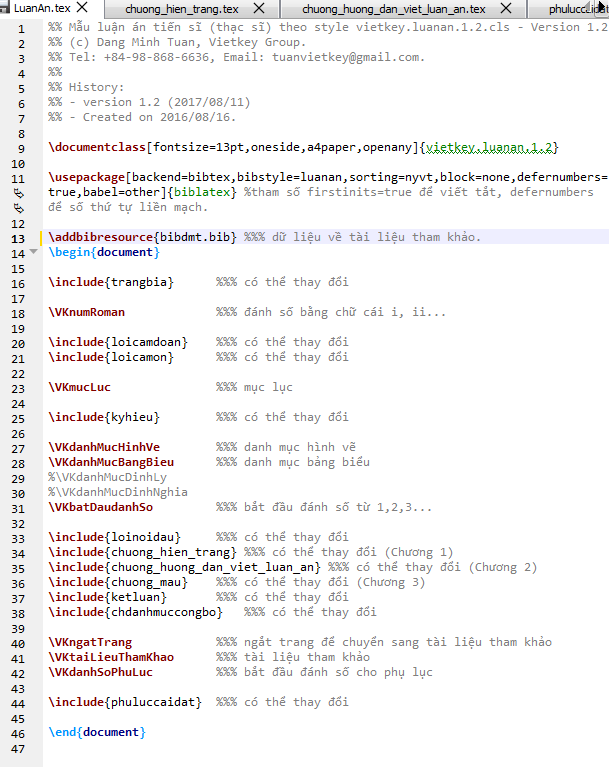
\includegraphics[scale=1.0]{master}
		\\		
	\end{center}	
	\caption{File gốc LuanAn.tex}	
	\label{h.goc}
\end{figure}

\subsection{Tài liệu tham khảo}

Ví dụ tham chiếu tài liệu tham khảo \cite{V10948}, hay \cite{V10944}, hoặc \cite{S10950}, và một số khác nữa: \cite{S9619}, \cite{S10950}. \cite{S10949}, \cite{S10791}, \cite{S10541}. \cite{S10921}, \cite{S556}, \cite{K02}.

Nhập liệu về tài liệu tham khảo trong file .bib như thường lệ xem file mẫu \textit{bibdmt.bib} đi kèm , tuy nhiên để có thể phân loại tài liệu tiếng Việt và tiếng Anh, chúng ta thêm hai trường là \textbf{langid = \{slovene\}} và \textbf{keywords = ``Vietnam''} để phân biệt với các văn bản tiếng Anh, có thể làm tương tự với tiếng Nga, tiếng Trung. \textit{Đáng tiếc là gói BibLaTex chưa hỗ trợ ngôn ngữ tiếng Việt do đó tác giả phải chọn ngôn ngữ \textit{slovene}} để tùy biến.

Ngoài ra ở trong file .bib có thể gõ tiếng Việt Unicode. Dưới đây là một mục (bài báo) trong file .bib có số liệu bằng tiếng Việt.
%\begin{lstlisting}[frame=trBL][language=TeX]{}

\textbf{Bài báo:}

\begin{tcolorbox}
\begin{verbatim}
@article{Bai22,
author    ="Nguyễn Hiếu Minh and Đỗ Thị Bắc",
title     ="{Một số lược đồ chữ ký số mù mới 
            dựa trên bài toán DLP và ECDLP}",
journal   ="Tạp Chí Khoa học và Công nghệ năm 2015",
volume    ="11",
number    ="5",
pages     ="3--11", 
year      ="2015",
langid    = {slovene},
keywords  = "Vietnam"
\end{verbatim}
\end{tcolorbox}

%\end{lstlisting}

\textbf{Sách:}

\begin{tcolorbox}
\begin{verbatim}
@book{V10945,
author ="Lưu Hồng Dũng",
title  ="Nghiên cứu, phát triển các lược đồ chữ ký số tập thể",
publisher ="Luận án tiến sĩ kỹ thuật, Học viện KTQS",
year ="2013",
keywords ="Vietnam"
\end{verbatim}
\end{tcolorbox}

\section{\bf Các gói đã được nhúng trong \textit{vietkey.luanan}}

\begin{itemize}
	\item \textbackslash usepackage[vietnam]\{babel\}
	\item \textbackslash usepackage[utf8]\{vietnam\}
	\item \textbackslash usepackage\{enumerate\}
	\item \textbackslash usepackage\{amsmath,amsxtra,amssymb,latexsym, amscd,amsthm\}
	\item \textbackslash usepackage\{indentfirst\}
	\item \textbackslash usepackage\{mathptmx\}
	\item \textbackslash usepackage\{fancyhdr\}
	\item \textbackslash usepackage\{picinpar\}
	\item \textbackslash usepackage\{floatflt\}
	\item \textbackslash usepackage\{epic\}
	\item \textbackslash usepackage\{curves\}
	\item \textbackslash usepackage\{makeidx\}
	\item \textbackslash usepackage\{longtable\}
	\item \textbackslash usepackage\{multicol\}
	\item \textbackslash usepackage\{listings\}
	\item \textbackslash usepackage[fontsize=13pt]\{scrextend\}
	\item \textbackslash usepackage[tight,vietnam]\{minitoc\}
	\item \textbackslash usepackage\{fancybox\}
	\item \textbackslash usepackage\{pdflscape\}
	\item \textbackslash usepackage\{tcolorbox\}
	\item \textbackslash usepackage\{enumitem\}  
	\item \textbackslash usepackage\{tikz\}
	\item \textbackslash usepackage[utf8]\{inputenc, vietnam\}
	\item \textbackslash usepackage\{color, graphicx\}
	\item \textbackslash usepackage[chapter]\{algorithm\}
	\item \textbackslash usepackage\{algorithmic\}
	\item \textbackslash usepackage\{eso-pic,calc\}
	\item \textbackslash usepackage\{hyperref\}
	\item \textbackslash usepackage\{bookmark\}
	\item \textbackslash usepackage\{titlesec\}
	\item \textbackslash usepackage\{thmtools\}
	\item \textbackslash usepackage\{booktabs\}
	\item \textbackslash usepackage\{geometry\}
	
\end{itemize}

\section{\bf Một số kinh nghiệm và lưu ý khi sử dụng}
\begin{itemize}
	\item Trong một số trường hợp khi cập nhật tài liệu tham khảo, việc đồng bộ giữa tham chiếu tài liệu tham khảo và dữ liệu tài liệu tham khảo có thể có sự khác biệt, khi đó cần phải xóa các file trung gian để phần mềm soạn thảo biên dịch lại từ đầu. Tác giả đã tạo ra một file chạy \textbf{clean.bat} tự động xóa hết các file này. Kích hoạt bằng cách nháy đúp con chuột vào file này trong File Explore.
	\item Tên các chương có thể được hiển thị khác nhau trong phần nội dung và phần mục lục. Trong phần nội dung do phải dùng font lớn để làm tiêu đề chương nên với tên dài cần phải ngắt dòng, tuy nhiên ở phần mục lục dùng font chữ nhỏ hơn nếu để tự động thì ở phần mục lục cũng ngắt dòng tương ứng như vậy sẽ không hợp lý. Để có thể hiển thị và ngắt dòng khác nhau có thể dùng dấu [] và \{\} sau lệnh \textbackslash chapter tương ứng với hiển thị trong mục lục và tiêu đề trong nội dung luận án.
\end{itemize}

\section{\bf Kết luận chương \ref{chchukytapthedathanhphan}}

\LaTeX\ nói chung và gói bilatex đang là xu thế được sử dụng để biên soạn luận án, luận văn và quản lý, sắp xếp tài liệu tham khảo một cách mềm dẻo và linh hoạt. Với class mới được phát triển ``\textbf{vietkey.luanan}'' có thể đáp ứng được hầu hết các yêu cầu trình bày luận án và cách sắp xếp và trích dẫn tài liệu tham khảo do các trường đại học ở Việt Nam quy định.

Mọi góp ý và đóng góp cho tài liệu cũng như gói class ``\textbf{vietkey.luanan}'' xin gửi về \textbf{tuanvietkey@gmail.com} hoặc thông qua \textbf{facebook.com/tuanvietkey}.

	%%% có thể thay đổi (Chương 2)
\chapter[CHƯƠNG MẪU-KẾT HỢP CHỮ KÝ SỐ TẬP THỂ ĐA THÀNH PHẦN VỚI CÁC MÔ HÌNH KHÁC]{KẾT HỢP CHỮ KÝ SỐ TẬP THỂ\\ ĐA THÀNH PHẦN VỚI CÁC MÔ HÌNH KHÁC} \label{chuchukykethop}  %
%\minitoc %
%\setcounter{baitap}{0}
%\thispagestyle{empty}
%\vspace*{1cm}
%%]-

%$Hash256(Hash256(blockHeaderWithoutNonce + nonce)) < target = 2^{(256-difficultyBits})$

Chương này đề xuất mô hình kết hợp giữa chữ ký số tập thể đa thành phần với chữ ký số ủy nhiệm và với chữ ký số mù. Ở mỗi loại hình kết hợp sẽ có lần lượt định nghĩa tổng quát, khả năng tấn công và đề xuất một lược đồ cụ thể để chứng minh tính đúng đắn của mô hình kết hợp.

\section{\bf Đề xuất mô hình chữ ký số tập thể đa thành phần}

\begin{figure}[ht]	
	\begin{center}		
		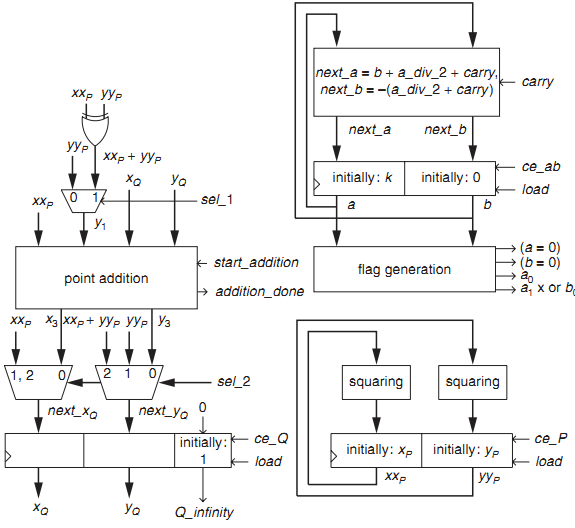
\includegraphics[scale=0.8]{nhanelliptic}
		\\		
	\end{center}	
	\caption{Phép nhân vô hướng trên đường cong elliptic}	
	\label{h.kytapthe33}
\end{figure}

Luận án đưa ra mô hình ký tập thể mới và gọi là \textit{Chữ ký số tập thể đa thành phần}. Ở đó mỗi thành viên có thể được giao cho nhiệm vụ ký một hay nhiều phần khác nhau của văn bản (các phần này không nhất thiết phải liên tục liền kề), mặt khác trong mô hình này, một thành phần của văn bản cũng có thể được một hay nhiều thành viên phụ trách và họ sẽ phải ký đồng thời vào thành phần này.


\begin{figure}[ht]	
	\begin{center}		
		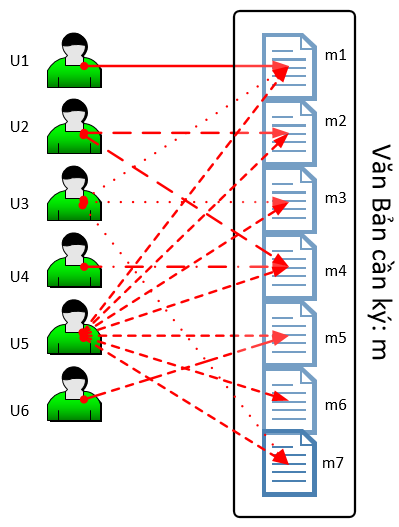
\includegraphics[scale=0.5]{kytapthe3}
		\\		
	\end{center}	
	\caption{Mô hình ký tập thể phân biệt trách nhiệm đa thành phần}	
	\label{h.kytapthe3}
\end{figure}

Hình \ref{h.kytapthe3} minh họa cho khái niệm chữ ký số tập thể đa thành phần. Ở đây có sáu người ký và văn bản được chia thành bảy phần khác nhau. Như vậy số thành viên ký trong tập thể và số thành phần văn bản được chia ra có tính độc lập tương đối với nhau. Số thành phần của văn bản có thể lớn hơn hay nhỏ hơn số thành viên của tập thể. 

Trong Hình \ref{h.kytapthe3}, có thể thấy vai trò và trách nhiệm ký của tập thể người ký như sau:
\begin{itemize}
	\item Các người ký $U1, U4, U6$ ký vào một phần của thông điệp $m$, tương ứng là các phần $m_1, m_4, m_5$.
	\item Người ký $U2$ ký và có trách nhiệm với 02 phần $m_2$ và $m_4$ của văn bản $m$.
	\item Người ký $U3$ có trách nhiệm ký với 03 phần $m_1, m_3, m_7$ của văn bản $m$.
	\item Người ký $U5$ có trách nhiệm ký tất cả các thành phần của văn bản $m$.
\end{itemize}

Mặt khác cũng trên Hình \ref{h.kytapthe3}, các thành phần của văn bản $m$ được ký bởi những người ký sau:
\begin{itemize}
	\item Thành phần $m_6$ chỉ do một người chịu trách nhiệm ký là $U5$.
	\item Các thành phần có 02 người chịu trách nhiệm ký là $m_2,m_3,m_5,m_7$.
	\item Riêng phần $m_4$ có 03 người chịu trách nhiệm ký là $U2,U4,U5$.
\end{itemize}

\begin{algorithm}%[H]
	\caption{Sinh chữ ký số ECDSA}
	INPUT: Tham số D = ($q$, FR, S, $a, b, P, n, h$), khóa bí mật $d$, thông điệp $m$. \\
	OUTPUT: Chữ ký số ($r, s$).
	\label{label1}
	\begin{algorithmic}[1]
		\STATE Chọn ngẫu nhiên $k \in [1, n-1],$ \label{tt.buoc1}
		\STATE  $R \gets kP=(x_1,y_1)$ và chuyển đổi $\bar{x_1}\gets x_1 $.
		\STATE  $r\gets\bar{x_1} \pmod n$.  
		\IF{$r=0$ or $R=\infty$} 
		\STATE Nhảy đến bước \ref{tt.buoc1}: 
		\ENDIF
		\STATE $e\gets H(m)$.
		\STATE $s \gets k^{-1}(e+dr) \pmod n$. 
		\IF{$s=0$}  
		\STATE Nhảy đến bước \ref{tt.buoc1}: 
		\ENDIF
		\STATE Trả về $(r,s)$
	\end{algorithmic}
\end{algorithm}


Đối với các tổ chức, cơ quan quản lý, văn bản $m$ có thể là công văn được phát ra, có nhiều thành phần liên quan đến chức năng của các phòng ban khác nhau trong tổ chức, có những thành phần sẽ liên quan chồng chéo giữa nhiều phòng ban và các phòng ban này phải chung nhau chịu trách nhiệm xem xét và ký duyệt.

Coi $\mathsf{NSIG}$ là tổng số các thành viên trong tập thể giam giá ký văn bản $m$, và $\mathsf{NSEC}$ là tổng số các thành phần cấu thành lên văn bản $m$. Tùy theo mối quan hệ và giá trị của $\mathsf{NSIG}$ và $\mathsf{NSEC}$ chúng ta có thể tổng hợp các mô hình ký văn bản trong Bảng \ref{bang1}. Quan sát bảng này chúng ta sẽ thấy: khi $\mathsf{NSEC}=\mathsf{NSIG}=1$ chúng ta sẽ có chữ ký số đơn. Trường hợp thứ 2 khi $\mathsf{NSIG}>1$ và $\mathsf{NSEC}=1$ chúng ta có mô hình chữ ký số tập thể không phân biệt trách nhiệm người ký. Trường hợp thứ 3 khi  $\mathsf{NSIG}>1$ và $\mathsf{NSIG}=\mathsf{NSEC}$ chúng ta có mô hình chữ ký số tập thể có phân biệt trách nhiệm người ký. Và cuối cùng là trường hợp thứ 4 khi $\mathsf{NSIG}$ và $\mathsf{NSEC}$ có giá trị bất kỳ. Qua Bảng \ref{bang1} chúng ta cũng dễ dàng nhận thấy mô hình ký tập thể đa thành phần mới được đề xuất là trường hợp tổng quát của tất cả các mô hình trước đó (ký đơn, ký tập thể không phân biệt trách nhiệm, ký tập thể có phân biệt trách nhiệm).

\begin{table}
	\centering
	\caption{Chữ ký số theo quan hệ giữa $\mathsf{NSIG}$ và $\mathsf{NSEC}$}
	\label{bang1}
	\begin{tabular}{l l p{6cm}}
		\toprule[0.125em]
		{\textsc{TT}} & {\textsc{Quan hệ}} & \textsc{{Mô hình chữ ký}}\\\toprule[0.125em]%\hline% \midrule
		1 & $\mathsf{NSIG}=1$ và $\mathsf{NSEC}=1$ & Mô hình chữ ký số đơn thông thường.\\  \midrule
		2 & $\mathsf{NSIG}>1$ và $\mathsf{NSEC}=1$ & Mô hình chữ ký số tập thể không phân biệt trách nhiệm người ký.\\\midrule
		3 & $\mathsf{NSIG}>1$ và $\mathsf{NSIG}=\mathsf{NSEC}$ & Mô hình chữ ký số tập thể phân biệt trách nhiệm người ký.\\\midrule
		4 & Với mọi $\mathsf{NSIG}$ và $\mathsf{NSEC}$  & Mô hình chữ ký số tập thể đa thành phần (có phân biệt trách nhiệm người ký).\\\bottomrule[0.125em]
	\end{tabular}
\end{table}

%\begin{center}
%	\begin{tabular}{||c c c c||} 
%		\hline
%		Col1 & Col2 & Col2 & Col3 \\ [0.5ex] 
%		\hline\hline
%		1 & 6 & 87837 & 787 \\ 
%		\hline
%		2 & 7 & 78 & 5415 \\
%		\hline
%		3 & 545 & 778 & 7507 \\
%		\hline
%		4 & 545 & 18744 & 7560 \\
%		\hline
%		5 & 88 & 788 & 6344 \\ [1ex] 
%		\hline
%	\end{tabular}
%\end{center}

\section{\bf Mô hình kết hợp chữ ký số tập thể đa thành phần và chữ ký số ủy nhiệm }

Chữ ký số ủy nhiệm là mô hình, lược đồ ký số mà ở đó một cá nhân có thể ủy quyền cho một cá nhân khác ký thay cho mình khi đi vắng. Và việc ký thay này có thể được gắn với một thuộc tính nào đó để hạn chế về điều kiện hiệu lực của việc ủy nhiệm, ví dụ như hạn chế về mặt thời gian, hạn chế về mặt nội dung, lĩnh vực ký.

\subsection{Định nghĩa chữ số tập thể ủy nhiệm đa thành phần tổng quát} \label{dnghiaTTUyNhiem}


Luận án đưa ra mô hình ký tập thể mới và gọi là \textit{Chữ ký số tập thể ủy nhiệm đa thành phần}. Ở đó mỗi thành viên có thể được giao cho nghiệm vụ ký một hay nhiều phần khác nhau của văn bản (các phần này không nhất thiết phải liên tục liền kề), mặt khác trong mô hình này, một thành phần của văn bản cũng có thể được một hay nhiều thành viên phụ trách và họ sẽ phải ký đồng thời vào thành phần này.

Giả sử có ${\mathsf{NSIG}}$ người ký $U_i$; $1\leqslant i\leqslant {\mathsf{NSIG}}$ cần ký văn bản $m \in  \{0,1\}^*$. Chia $m$ thành $\mathsf{NSEC}$ phần, sao cho có thể biểu diễn $m$ dưới dạng: \[ m= (m_1\parallel m_2\parallel m_3 \parallel \dotsm \parallel m_\mathsf{NSEC} ). \] sử dụng ký hiệu và định nghĩa mảng phân công ký $\mathfrak{V}$.

Từng thành viên $U_i$ sẽ chịu trách nhiệm ký một số phần của văn bản $m$, tính giá trị hàm băm $h_i(m_j)$; $1\leqslant j\leqslant \mathsf{NSEC}$ và gửi cho người ủy nhiệm, người này sẽ tính giá trị băm tổng hợp $H_e$. 

\begin{defi}[Chữ ký số tập thể ủy nhiệm đa thành phần - MSMS-PROXY] Giả sử văn bản $m$ được chia thành $ \mathsf{NSEC}$, có tập thể $ \mathsf{NOSIG}$ người ủy nhiệm cần ủy nhiệm quyền ký cho tập thể $ \mathsf{NPSIG}$ người ký, chữ ký tập thể ủy nhiệm đa thành phần là tập bộ 13 thành phần ($\boldsymbol{\mathsf{Setup}}$, $\boldsymbol{\mathsf{KeyGen}_{OSIG}}$, $\boldsymbol{\mathsf{KeyGenPub}_{OSIG}}$, $\boldsymbol{\mathsf{Sign}_{OSIG}}$, $\boldsymbol{\mathsf{SignPub}_{OSIG}}$, $\boldsymbol{\mathsf{Verify}_{OSIG}}$, $\boldsymbol{\mathsf{VerifyPub}_{OSIG}}$,  $\boldsymbol{\mathsf{KeyGen}_{PSIG}}$, $\boldsymbol{\mathsf{KeyGenPub}_{PSIG}}$, $\boldsymbol{\mathsf{Sign}_{PSIG}}$, $\boldsymbol{\mathsf{SignPub}_{PSIG}}$, $\boldsymbol{\mathsf{Verify}_{PSIG}}$, $\boldsymbol{\mathsf{VerifyPub}_{PSIG}}$ )  có thuật toán thực hiện trong thời gia đa thức với các giao thức sau:  \label{dn311}

\begin{enumerate}[label=(\arabic*)]
	\item Khởi tạo tham số $\mathsf{params} $ với $k$ là tham số độ an toàn, $R$ là tham số ngẫu nhiên.
	\begin{equation}
	\mathsf{params} \stackrel{R}{\longleftarrow}  \boldsymbol{\mathsf{Setup}}(1^k)
	\end{equation}
	\item Sinh khóa công khai và bí mật cho các thành viên $OSIG_i$, $1\leqslant i\leqslant \mathsf{NOSIG}$.
	\begin{equation}
	\mathsf{(PK.OSIG_i,SK.OSIG_i)} \gets \boldsymbol{\mathsf{KeyGen}_{OSIG}}(\mathsf{params},1^k, i)
	\end{equation}
	Sau khi có khóa công khai của từng thành viên, sinh khóa công khai của cả tập thể bằng thuật toán:
	\begin{equation}
	\mathsf{(PK.OSIG_{pub})} \gets \{\boldsymbol{\mathsf{KeyGenPub}_{OSIG}}(\mathsf{PK.OSIG_i})\}^{\mathsf{NOSIG}}_{i=1}
	\end{equation}	
	\item Hình thành chữ ký của tập thể người ủy nhiệm: Từng thành viên $OSIG_i$ tham gia ký văn bản theo thuật toán dưới đây:
	\begin{equation}
	\sigma.OSIG_i \gets \boldsymbol{\mathsf{Sign}_{OSIG}}^R(\mathtt{SK.OSIG_i},m)
	\end{equation}
	Người tổng hợp cần phải kiểm tra chữ ký của từng thành viên bằng thuật toán sau:
	\begin{equation}
	\{0,1\} \gets \{\boldsymbol{\mathsf{Verify}_{OSIG}}(\mathsf{PK.OSIG_{i}},m,\sigma_{i})\}^{\mathsf{NOSIG}}_{i=1}  
	\end{equation}
	Nếu tất cả đều hợp lệ (Accept) thì tiến hành tính chữ ký của cả tập thể, nếu không thì yêu cầu thực hiện lại bước này.
	\begin{equation}
	\sigma.OSIG_{pub} \gets \{\boldsymbol{\mathsf{SignPub}_{OSIG}}^R(\sigma_i)\}^{\mathsf{NOSIG}}_{i=1}
	\end{equation}
	\item Xác thực văn bản của tập thể người ủy nhiệm:
	\begin{equation}
	\{0,1\} \gets \boldsymbol{\mathsf{VerifyPub}_{OSIG}}(\mathsf{PK.OSIG_{pub}},m',\sigma.OSIG_{pub})  
	\end{equation}
	\item Sinh khóa công khai và bí mật cho các thành viên được ủy nhiệm $PSIG_j$, $1\leqslant j\leqslant \mathsf{NPSIC}$, $w$ là giá trị bảo đảm.
	\begin{equation}
	\mathsf{(PK.PSIG_j,SK.PSIG_j)} \gets \boldsymbol{\mathsf{KeyGen}_{PSIG}}(\mathsf{params},w, 1^k, j, \mathfrak{V}_j)
	\end{equation}
	Sau khi có khóa công khai của từng thành viên, sinh khóa công khai của cả tập thể bằng thuật toán:
	\begin{equation}
	\mathsf{(PK.PSIG_{pub})} \gets \{\boldsymbol{\mathsf{KeyGenPub}_{PSIG}}(\mathsf{PK.PSIG_j},\mathfrak{V}_j)\}^{\mathsf{NPSIC}}_{j=1}
	\end{equation}	
	\item Hình thành chữ ký của tập thể người ủy nhiệm: Từng thành viên $PSIG_j$ tham gia ký văn bản theo thuật toán dưới đây:
	\begin{equation}
	\sigma.PSIG_j \gets \boldsymbol{\mathsf{Sign}_{PSIG}}^R(\mathtt{SK.PSIG_j},w,m,\mathfrak{V}_j)
	\end{equation}
	Người tổng hợp cần phải kiểm tra chữ ký của từng thành viên bằng thuật toán sau:
	\begin{equation}
	\{0,1\} \gets \{\boldsymbol{\mathsf{Verify}_{PSIG}}(\mathsf{PK.PSIG_{j}},w,m,\sigma_{j},\mathfrak{V}_j)\}^{\mathsf{NPSIC}}_{j=1} 
	\end{equation}
	Nếu tất cả đều hợp lệ (Accept) thì tiến hành tính chữ ký của cả tập thể, nếu không thì yêu cầu thực hiện lại bước này.
	\begin{equation}
	\sigma.PSIG_{pub} \gets \{\boldsymbol{\mathsf{SignPub}_{PSIG}}^R(\sigma_j,\mathfrak{V})\}^{\mathsf{NPSIC}}_{j=1}
	\end{equation}
	\item Xác thực văn bản của tập thể người được ủy nhiệm:
	\begin{equation}
	\{0,1\} \gets \boldsymbol{\mathsf{VerifyPub}_{PSIG}}(\mathsf{PK.PSIG_{pub}},m',\sigma.PSIG_{pub})  
	\end{equation}
\end{enumerate}
\end{defi}


\subsection{Tấn công ACMA - Adaptive Chosen Message Attacks với mô hình MSMS-PROXY}

Đây là loại hình tấn công mạnh nhất, kẻ tấn công có thể được lựa chọn văn bản để ký phụ thuộc vào khóa công khai cũng như những chữ ký số có từ trước đó. Có thể biểu diễn việc này thông qua khả năng truy cập đến hàm Oracle, ký hiệu là $\mathsf{Sign(\cdot)}_{sk}$.

%\begin{landscape}
\begin{equation}
 \arraycolsep=1.4pt\def\arraystretch{1.7} %giãn dòng trong \begin{array}
 \resizebox{1.11\hsize}{!}{$% bóp công thức nhỏ đi
\epsilon_{\mathcal{A}}(k) \eqdefU \Pr
\left[ 
%\left( 
\begin{array}{c}
\{m_{i_m}\}^{\ell}_{i_m=1} \gets M_k;\\
\mathsf{(PK.OSIG_i,SK.OSIG_i)} \gets \boldsymbol{\mathsf{KeyGen}_{OSIG}}(\mathsf{params},1^k, i) ; \\
	\mathsf{(PK.OSIG_{pub})} \gets\{\boldsymbol{\mathsf{KeyGenPub}_{OSIG}}(\mathsf{PK.OSIG_i})\}^{\mathsf{NOSIG}}_{i=1};\\
\sigma.OSIG_i \gets \boldsymbol{\mathsf{Sign}_{OSIG}}^R(\mathtt{SK.OSIG_i},m);\\
\mathsf{(PK.PSIG_j,SK.PSIG_j)} \gets \boldsymbol{\mathsf{KeyGen}_{PSIG}}(\mathsf{params},w, 1^k, j, \mathfrak{V}_j) ; \\
\mathsf{(PK.PSIG_{pub})} \gets \{\boldsymbol{\mathsf{KeyGenPub}_{PSIG}}(\mathsf{PK.PSIG_j},\mathfrak{V}_j)\}^{\mathsf{NPSIC}}_{j=1} ;\\
\sigma.PSIG_j \gets \boldsymbol{\mathsf{Sign}_{PSIG}}^R(\mathtt{SK.PSIG_j},w,m,\mathfrak{V}_j);\\
\sigma.PSIG_{{pub}_{i_m}} \gets \{\boldsymbol{\mathsf{SignPub}_{PSIG}}^R(\sigma_j,\mathfrak{V})\}^{\mathsf{NPSIC}}_{j=1};\\
(m,\sigma.PSIG_{{pub}_{i_m}}) \gets \mathcal{A}^{\mathsf{Sign(\cdot)}_{sk}}\left( \mathsf{PK_{pub}}\right) 
\end{array} 
%\right) 
:
\begin{array}{c}
%1 \gets \left\lbrace \boldsymbol{\mathsf{Verify}}(\mathsf{PK_{i}},m,\sigma_{i},\mathfrak{V}_i)\right\rbrace_{i=1}^{\mathsf{NSIG}} ;\\
1 \gets \boldsymbol{\mathsf{VerifyPub}}(\mathsf{PK_{pub}},m,\sigma_{pub},\mathfrak{V}) \\
\wedge \quad m \notin \{m_1,\ldots,m_{\ell}\}
\end{array}
\right] 
$}
\end{equation}
\[ 
\epsilon_{\mathcal{A}}(k) \le \mathsf{negl}(k)
 \]
\begin{defi} Lược đồ MSMS-PROXY được cho là không thể giả mạo với tấn công ACMA khi với mọi thuật toán thời gian đa thức của người tấn công $\mathcal{A}$, xác suất thành công của thực nghiệm dưới đây là một hàm nhỏ không đáng kể:
	\begin{enumerate}[label=(\arabic*)]
		\item Chuỗi $\ell=\ell(k)$ văn bản $m_1,\ldots,m_{\ell}$ được chọn một cách ngẫu nhiên trong không gian $M_k$.
		\item Thực hiện các thuật toán trong lược đồ để tạo ra chữ ký $\sigma_{{pub}_{i_m}}$.
		\item Thuật toán $\mathcal{A}$ với đầu vào là $\mathsf{PK_{pub}}$ và có thể truy cập đến $\mathsf{Sign(\cdot)}_{sk}$ với một số văn bản bất kỳ và sẽ cho ra chữ ký số $(m,\sigma_{pub}) $. Không gian các văn bản truy vấn này gọi là $M$.
		\item Thực nghiệm tấn công thành công nếu $1 \gets \boldsymbol{\mathsf{VerifyPub}}(\mathsf{PK_{pub}},m,\sigma_{pub},\mathfrak{V})$ và $m\ne M$.
	\end{enumerate}	
\end{defi}
%\end{landscape}

\subsection{Đề xuất chữ ký số tập thể đa thành phần ủy nhiệm dựa trên hệ mật định danh} \label{muc.uynhiemIDBased}

%Do Rajeev Anand và Sahadeo Padhye đề xuất vào năm 2013 \cite{S10851}.

\subsubsection {Cài đặt}
Coi $G_1$ là nhóm cộng cyclic có bậc là số nguyên tố $q$ và phần tử sinh là $P$. $G_2$ là nhóm nhân cyclic có cùng bậc $q$. $e$ là một ánh xạ song tuyến tính: \[ \hat{e}: G_1 \times G_1 \to G_2 \] $H_1, H_2, H_3$ là các hàm băm được sử dụng cho mục đích bảo mật và được định nghĩa như sau:
\begin{align}
	H_1: \{0,1\}^* & \to G_1 \\
	H_2: \{0,1\}^* & \to \mathbb{Z}_q^* \\
	H_3: \{0,1\}^* \times \{0,1\}^* & \to \mathbb{Z}_q^*
\end{align}


\begin{enumerate}[label=(\arabic*)]
	\item Với tham số bảo mật $k$ chọn ngẫu nhiên $s \in \mathbb{Z}_q^*$.
	\item Tính khóa công khai của hệ thống: \[ P_{pub} = sP \in G_1 \]
	\item Công bố tham số của hệ thống là: \[ Params = (k,G_1,G_2,q,\hat{e},H_1,H_2,H_3, P,P_{pub}) \]
\end{enumerate}	

\subsubsection{Tách khóa}

Người ký ủy nhiệm có định danh là $ID$, có $\mathsf{NPSIC}$ người có thể ký ủy nhiệm $ID_{B_i}$ với $1\le i \le \mathsf{NPSIC}$.
\begin{enumerate}[label=(\arabic*)]
	\item Bất kỳ ai cũng có thể tính khóa công khai của người cần ủy nhiệm: 
	\[ Q_{ID} = H_1(ID) \in G_1 \] và những người được ủy nhiệm: \[ Q_{ID_{B_i}} = H_1(ID_{B_i}) \in G_1 \]
	\item Người quản trị hệ thống sẽ tính khóa bí mật cho người ủy nhiệm và được ủy nhiệm:
	\begin{align*}
		S_{ID} &= sQ_{ID} \\
		S_{ID_{B_i}} &= sQ_{ID_{B_i}} \quad 1\le i \le \mathsf{NPSIC}
	\end{align*}
	Người quản trị sẽ thông qua kênh bí mật gửi các khóa bí mật này cho các thành viên.
\end{enumerate}

\subsubsection{Hình thành chữ ký của người ủy nhiệm}

\begin{enumerate}[label=(\arabic*)]
	\item Với văn bản $m \in \{0,1\}^*$, người ký chọn ngẫu nhiên $x \in \mathbb{Z}_q^*$.
	\item Tính các giá trị:
	\begin{align*}
	V_s &= xP\\
	H &=H_2(m) \\
	W_s &= HS_{ID} + xP_{pub}
	\end{align*}
	\item chữ ký của người ủy nhiệm là $\sigma = (W_s,V_s)$.
\end{enumerate}	

\subsubsection{Xác thực chữ ký người ủy nhiệm}

\begin{enumerate}[label=(\arabic*)]
	\item Với văn bản $m'$ và chữ ký $\sigma = (W_s,V_s)$ nhận được, người xác thực tính: 
	 \[ H'=H_2(m') \]  \[ Q_{ID} = H_1(ID) \]
	\item Chấp nhận chữ ký khi điều kiện sau thỏa mãn:
	\begin{equation}
	\hat{e}(W_s,P) = \hat{e}(H'Q_{ID} + V_s,P_{pub})
	\end{equation}
\end{enumerate}

\subsubsection{Sinh khóa cho người được ủy nhiệm}

Trong giai đoạn này người ủy nhiệm sẽ trao đổi với người được ủy nhiệm với các quyền được ủy nhiệm. Để làm việc này người ủy nhiệm sẽ tạo ra một văn bản bảo đảm $w$, văn bản này sẽ kèm theo một số thông tin về văn bản, về những hạn chế của văn bản sẽ ủy nhiệm, thời gian hoặc định danh của những người sẽ ủy nhiệm.
\begin{enumerate}[label=(\arabic*)]
	\item \textit{Ủy nhiệm}: Người cần ủy nhiệm chọn ngẫu nhiên $t \in \mathbb{Z}_q^*$ và tính:
	\begin{align*}
	V &= tP, \\
	h &=H_2(w), \\
	W &= hS_{ID} + tP_{pub} \in G_1
	\end{align*}
	Chuyển giá trị $(W, V, w)$ với các thành viên qua kênh truyền bí mật.
	\item \textit{Kiểm tra ủy nhiệm}: mỗi thành viên $ID_{B_i}$ sẽ tính $ h =H_2(w) $ và kiểm tra điều kiện sau (nếu không thỏa mãn thì phải yêu cầu gửi lại hoặc hủy giao thức):
	\begin{equation*}
	\hat{e}(W,P) = \hat{e}(hQ_{ID} + V,P_{pub})
	\end{equation*}
	\item \textit{Sinh khóa ủy nhiệm}: mỗi thành viên $ID_{B_i}$ sẽ tính $ h =H_2(w) $ tính khóa bí mật ủy nhiệm:
	\begin{equation*}
	S_{pk_i} = W + hS_{ID_{B_i}}
	\end{equation*}
\end{enumerate}

\subsubsection{Hình thành chữ ký ủy nhiệm}
Trong pha này sẽ có một người phụ trách có nhiệm vụ tập hợp hết tất cả các chữ ký thành phần.


\begin{enumerate}[label=(\arabic*)]
	%\item Mỗi thành viên $ID_{B_i}$ sẽ chọn ngẫu nhiên số $x_i \in \mathbb{Z}_q^*$.
	\item Mỗi thành viên $ID_{B_i}$ ($1\leqslant i\leqslant \mathsf{NPSIC}$) chọn ngẫu nhiên số nguyên $x_i\in Z_q^*$ như là khóa bí mật và tính khóa công khai tương ứng theo công thức: 
	\begin{equation}
	U_{p_i}=x_iP
	\end{equation}
%	với định nghĩa phép toán:        
%	\begin{equation}
%	\mathfrak{V}_i \otimes x_i=\sum_{j=1}^\mathsf{NSEC} (\mathfrak{V}_{i}[j]\times x_{i}[j]) \pmod q 
%	\end{equation}
	Giả thiết có $\mathsf{NPSIC}$ người $ID_{B_i}$; $1\leqslant i\leqslant \mathsf{NPSIC}$ cần ký văn bản $m \in  \{0,1\}^*$. Chia văn bản $m$ thành $\mathsf{NSEC}$ phần, sao cho có thể viết $m$ theo dạng \[ m= (m_1|| m_2|| m_3 || \dots || m_\mathsf{NSEC} ) \] sử dụng ký hiệu và định nghĩa mảng phân công ký $\mathfrak{V}$ như ở Định nghĩa \ref{mangKy} (trang \pageref{mangKy}).
	
	Từng thành viên $ID_{B_i}$ sẽ chịu trách nhiệm ký một số phần của văn bản $m$, tính giá trị hàm băm $h_i(m_j)$; $1\leqslant j\leqslant \mathsf{NSEC}$ và gửi cho người ủy nhiệm, người này sẽ tính giá trị băm cho $m_j$ như sau:
	\begin{align}
	e_j &=\sum_{i=1}^{\mathsf{NSIG}} \left(\mathfrak{V}_i[j] \times h_i(m_j)\right); \quad 1\leqslant j\leqslant \mathsf{NSEC} \\
	h_3 &=H_3(e_1||e_2\cdots ||e_\mathsf{NSEC},w)
	\end{align}	
	Bằng cách tính như trên chúng ta thu được chữ ký số tập thể có phân biệt trách nhiệm, gửi giá trị $U_{p_i}$ đến $(\mathsf{NPSIC}-1)$ các thành viên còn lại.
	\item Các thành viên tính và gửi $ \sigma_{p_i} $ :
	\begin{align*}
	U_p &=\sum_{i=1}^{\mathsf{NPSIG}}U_{p_i} \\
	\sigma_{p_i} &= h_3S_{pk_i} + x_iP_{pub}
	\end{align*}
	\item Người phụ trách sau khi có các chữ ký thành phần sẽ tạo khóa công khai ủy nhiệm:
	\begin{equation}
	Q_{pk_i} = h\left(Q_{ID} + Q_{ID_{B_i}} \right)  + V
	\end{equation}
	Và sau đó kiểm tra điều kiện:
	\begin{align}
	\hat{e}(P,\sigma_{p_i}) &= \hat{e}(P_{pub},h'Q_{pk_i} + U_{p_i}) \\
	\sigma_p &=\sum_{i=1}^{\mathsf{NPSIG}}\sigma_{p_i}
	\end{align}
	sau đó chữ ký số ủy nhiệm sẽ là $(\sigma_p,V,w,U_p,\mathfrak{V})$.
\end{enumerate}

\subsubsection{Xác thực chữ ký ủy nhiệm}
Người xác thực chữ ký ủy nhiệm sau khi nhận văn bản $m'$ và chữ ký  $(\sigma_p,V,w,U_p,\mathfrak{V})$ sẽ tiến hành các bước sau:
\begin{enumerate}[label=(\arabic*)]
	\item Kiểm tra $m'$ và bảo đảm $w$ và các điều kiện liên quan.
	\item Kiểm tra sự ủy quyền của $\mathsf{NPSIG}$ người ký. Nếu không hợp lệ thì dựng lại và từ chối chữ ký.
	\item Tính các giá trị:
	\begin{align*}
	h &=H_2(w) \\
	h_3' &= H_3(m',w) \\
	Q_{pk} &= h\left[ \mathsf{NPSIG}\cdot Q_{ID} + \sum_{i=1}^{\mathsf{NPSIG}}Q_{ID_{B_i}} \right]  + \mathsf{NPSIG} \cdot V
	\end{align*}
	\item Kiểm tra điều kiện sau nếu đúng thì chấp nhận chữ ký, ngược lại là từ chối chữ ký:
	\begin{equation}
	\hat{e}(P,\sigma_p)  = \hat{e}(P_{pub},h_3'Q_{pk} + U_p)
	\end{equation}
\end{enumerate}

\begin{theorem}[Lược đồ ký tập thể ủy nhiệm đa thành phần]
	Nếu $m'=m$ thì $\hat{e}(P,\sigma_p)  = \hat{e}(P_{pub},h_3'Q_{pk} + U_p)$.
\end{theorem}

\begin{proof}
	\begin{align*}
	\hat{e}(P,\sigma_p)  &= \hat{e}(P_{pub},h_3'Q_{pk} + U_p) \\
	\hat{e}(P,\sum_{i=1}^{\mathsf{NPSIG}}\sigma_{p_i}) &= \hat{e}(P_{pub},h_3'Q_{pk} + U_p) \\
	\hat{e}(P,\sum_{i=1}^{\mathsf{NPSIG}} \left[ h_3S_{pk_i} + x_iP_{pub} \right] ) &= \hat{e}(P_{pub},h_3'Q_{pk} + U_p) \\
	\hat{e}(P,\sum_{i=1}^{\mathsf{NPSIG}}\left[ h_3\left(W + hS_{ID_{B_i}} \right)  + x_iP_{pub} \right]) &= \hat{e}(P_{pub},h_3'Q_{pk} + U_p) \\
	\hat{e}(P,\sum_{i=1}^{\mathsf{NPSIG}}\left[ h_3\left(hS_{ID} + tP_{pub} + hS_{ID_{B_i}} \right)  + x_iP_{pub} \right]) &= \hat{e}(P_{pub},h_3'Q_{pk} + U_p) \\
	\hat{e}(P,\sum_{i=1}^{\mathsf{NPSIG}}\left[ h_3\left(hsQ_{ID} + tsP + hsQ_{ID_{B_i}} \right)  + x_isP \right]) &= \hat{e}(P_{pub},h_3'Q_{pk} + U_p) \\
	\hat{e}(P_{pub},\sum_{i=1}^{\mathsf{NPSIG}}\left[ h_3\left(hQ_{ID} + tP + hQ_{ID_{B_i}} \right)  + x_iP \right]) &= \hat{e}(P_{pub},h_3'Q_{pk} + U_p) \\
	\hat{e}(P_{pub},\sum_{i=1}^{\mathsf{NPSIG}}\left[ h_3\left(hQ_{ID} + V + hQ_{ID_{B_i}} \right) \right]+ U_p) &= \hat{e}(P_{pub},h_3'Q_{pk} + U_p) \\
	\hat{e}(P_{pub},h_3\left[\sum_{i=1}^{\mathsf{NPSIG}} \left(hQ_{ID_{B_i}} \right) + \mathsf{NPSIG}\cdot hQ_{ID} + \mathsf{NPSIG}\cdot V \right] + U_p) &= \hat{e}(P_{pub},h_3'Q_{pk} + U_p) \\
	\hat{e}(P_{pub},h_3\left[h\left[ \mathsf{NPSIG}\cdot Q_{ID} + \sum_{i=1}^{\mathsf{NPSIG}} Q_{ID_{B_i}}\right]  + \mathsf{NPSIG}\cdot V \right] + U_p) &= \hat{e}(P_{pub},h_3'Q_{pk} + U_p)\\
	\hat{e}(P_{pub},h_3Q_{pk} + U_p) &= \hat{e}(P_{pub},h_3'Q_{pk} + U_p)
	\end{align*}
	Biểu thức cuối cùng đúng khi $h_3' = h_3$.	
\end{proof}

Phần phân tích hiệu năng và an toàn của lược đồ đề xuất theo mô hình an toàn đã định nghĩa rất dài và vì chương này chỉ mang tính minh họa cho việc kết hợp mô hình chữ ký số tập thể đa thành phần với mô hình chữ ký khác nên không được trình bày cụ thể ở đây.

\section{\bf Mô hình kết hợp chữ ký số tập thể đa thành phần và chữ ký số mù}

\subsection{Định nghĩa chữ ký số tập thể mù đa thành phần tổng quát} \label{dnghiaTTMu}


Luận án đưa ra mô hình ký tập thể mới và gọi là \textit{Chữ ký số tập thể mù đa thành phần}. Ở đó mỗi thành viên có thể được giao cho nghiệm vụ ký một hay nhiều phần khác nhau của văn bản (các phần này không nhất thiết phải liên tục liền kề), mặt khác trong mô hình này, một thành phần của văn bản cũng có thể được một hay nhiều thành viên phụ trách và họ sẽ phải ký đồng thời vào thành phần này.

Giả sử có $\mathsf{NSIG}$ người ký $U_i$; $1\leqslant i\leqslant \mathsf{NSIG}$ cần ký văn bản $m \in  \{0,1\}^*$. Chia $m$ thành $\mathsf{NSEC}$ phần, sao cho có thể biểu diễn $m$ dưới dạng:\[  m= (m_1\parallel m_2\parallel m_3 \parallel \dotsm \parallel m_\mathsf{NSEC} ) \] Sử dụng ký hiệu và định nghĩa mảng phân công ký $\mathfrak{V}$.

Từng thành viên $U_i$ sẽ chịu trách nhiệm ký một số phần của văn bản $m$, tính giá trị hàm băm $h_i(m_j)$; $1\leqslant j\leqslant \mathsf{NSEC}$ và gửi cho người ủy nhiệm, người này sẽ tính giá trị băm tổng hợp $H_e$ như Định nghĩa. 
 
\begin{defi}[Chữ ký số tập thể mù đa thành phần] Lược đồ chữ ký số tập thể đa thành phần là tập bộ 09 thành phần ($\boldsymbol{\mathsf{Setup}}$, $\boldsymbol{\mathsf{KeyGen}}$, $\boldsymbol{\mathsf{KeyGenPub}}$, $\boldsymbol{\mathsf{Blind}}$, $\boldsymbol{\mathsf{Sign}}$, $\boldsymbol{\mathsf{SignPub}}$, $\boldsymbol{\mathsf{UnBlid}}$, $\boldsymbol{\mathsf{Verify}}$, $\boldsymbol{\mathsf{VerifyPub}}$) có thuật toán thực hiện trong thời gia đa thức và có giao thức giữa các thành phần như sau: 
	
	\begin{enumerate}[label=(\arabic*)]
		\item Bộ khởi tạo $\boldsymbol{\mathsf{Setup}}$: đầu ra là bộ tham số $\mathsf{params} $ 
		\begin{equation}
		\mathsf{params} \stackrel{R}{\longleftarrow}  \boldsymbol{\mathsf{Setup}}(1^k)
		\end{equation}
		\item Sinh khóa công khai và bí mật cho các thành viên $U_i$, $1\leqslant i\leqslant \mathsf{NSIG}$.
		\begin{equation}
		\mathsf{(PK_i,SK_i)} \gets \boldsymbol{\mathsf{KeyGen}}(\mathsf{params},1^k, i)
		\end{equation}
		Sau khi có khóa công khai của từng thành viên, sinh khóa công khai của cả tập thể bằng thuật toán:
		\begin{equation}
		\mathsf{(PK_{pub})} \gets \{\boldsymbol{\mathsf{KeyGenPub}}(\mathsf{PK_i},\mathfrak{V}_i)\}^{\mathsf{NSIG}}_{i=1}
		\end{equation}	
		\item Người cần ký $\boldsymbol{\mathcal{U}}$ mã hóa văn bản $m$ để tạo ra bản mã $\overline{m}$ bằng thuật toán $\boldsymbol{\mathsf{Blind}}$:
		\begin{equation}
		\overline{m} \gets \{\boldsymbol{\mathsf{Blind}}(m,\mathsf{PK_i})\}^{\mathsf{NSIG}}_{i=1}
		\end{equation}
		\item Ký văn bản: Từng thành viên $U_i$ tham gia ký văn bản theo thuật toán dưới đây:
		\begin{equation}
		\overline{\sigma}_i \gets \boldsymbol{\mathsf{Sign}}^R(\mathtt{SK_i},\overline{m},\mathfrak{V}_i)
		\end{equation}
		Người tổng hợp cần phải kiểm tra chữ ký của từng thành viên bằng thuật toán sau:
		\begin{equation}
		\{0,1\} \gets \{\boldsymbol{\mathsf{Verify}}(\mathsf{PK_{i}},m,\sigma_{i},\mathfrak{V}_i)\}^{\mathsf{NSIG}}_{i=1}  
		\end{equation}
		Nếu tất cả đều hợp lệ (Accept) thì tiến hành tính chữ ký của cả tập thể, nếu không thì yêu cầu thực hiện lại bước này.
		\begin{equation}
		\overline{\sigma}_{pub} \gets \{\boldsymbol{\mathsf{SignPub}}^R(\overline{\sigma}_i)\}^{\mathsf{NSIG}}_{i=1}
		\end{equation}
		\item Người cần ký $\boldsymbol{\mathcal{U}}$ xóa mù cho chữ ký tập thể:
		\begin{equation}
		\sigma_{pub} \gets \{\boldsymbol{\mathsf{UnBlind}}^R(\overline{\sigma}_{pub},\mathsf{PK_i})\}^{\mathsf{NSIG}}_{i=1}
		\end{equation}
		\item Xác thực văn bản:
		\begin{equation}
		\{0,1\} \gets \boldsymbol{\mathsf{VerifyPub}}(\mathsf{PK_{pub}},m',\sigma_{pub},,\mathfrak{V})  
		\end{equation}
	\end{enumerate}
\end{defi}

\subsection{Tấn công ACMA - Adaptive Chosen Message Attacks với mô hình MSMS-BL}
Đây là loại hình tấn công mạnh nhất, kẻ tấn công có thể được lựa chọn văn bản để ký phụ thuộc vào khóa công khai cũng như những chữ ký số có từ trước đó. Có thể biểu diễn việc này thông qua khả năng truy cập đến hàm Oracle, ký hiệu là $\mathsf{Sign(\cdot)}_{sk}$.

%\begin{landscape}
\[ \arraycolsep=1.4pt\def\arraystretch{1.7} %giãn dòng trong \begin{array}
\epsilon_{\mathcal{A}}(k) \eqdefU \Pr
\left[ 
%\left( 
\begin{array}{c}
\{m_{i_m}\}^{\ell}_{i_m=1} \gets M_k;\\
\left\lbrace \mathsf{(PK_i,SK_i)}\gets \boldsymbol{\mathsf{Gen}}(\mathsf{params},1^k)\right\rbrace_{i=1}^{\mathsf{NSIG}} ; \\
\mathsf{PK_{pub}} \gets \left\lbrace \boldsymbol{\mathsf{GenPub}}(\mathsf{PK_i},\mathfrak{V}_i)\right\rbrace_{i=1}^{\mathsf{NSIG}} ;\\
\overline{m} \gets \{\boldsymbol{\mathsf{Blind}}(m,\mathsf{PK_i})\}^{\mathsf{NSIG}}_{i=1}; \\
\overline{\sigma}_i \gets \boldsymbol{\mathsf{Sign}}^R(\mathtt{SK_i},\overline{m},\mathfrak{V}_i) ;\\
\overline{\sigma}_{pub} \gets \{\boldsymbol{\mathsf{SignPub}}^R(\overline{\sigma}_i)\}^{\mathsf{NSIG}}_{i=1} ;\\
\sigma_{{pub}_{i_m}} \gets \{\boldsymbol{\mathsf{UnBlind}}^R(\overline{\sigma}_{pub},\mathsf{PK_i})\}^{\mathsf{NSIG}}_{i=1} ;\\
(m,\sigma_{pub}) \gets \mathcal{A}^{\mathsf{Sign(\cdot)}_{sk}}\left( \mathsf{PK_{pub}}\right) 
\end{array} 
%\right) 
:
\begin{array}{c}
%1 \gets \left\lbrace \boldsymbol{\mathsf{Verify}}(\mathsf{PK_{i}},m,\sigma_{i},\mathfrak{V}_i)\right\rbrace_{i=1}^{\mathsf{NSIG}} ;\\
1 \gets \boldsymbol{\mathsf{VerifyPub}}(\mathsf{PK_{pub}},m,\sigma_{pub},\mathfrak{V}) \\
\wedge \quad m \notin \{m_1,\ldots,m_{\ell}\}
\end{array}
\right]
\] 
\[ 
\epsilon_{\mathcal{A}}(k) \le \mathsf{negl}(k)
\] 
\begin{defi} Lược đồ MSMS được cho là không thể giả mạo với tấn công ACMA khi với mọi thuật toán thời gian đa thức của người tấn công $\mathcal{A}$, xác suất thành công của thực nghiệm dưới đây là một hàm nhỏ không đáng kể:
	\begin{enumerate}[label=(\arabic*)]
		\item Chuỗi $\ell=\ell(k)$ văn bản $m_1,\ldots,m_{\ell}$ được chọn một cách ngẫu nhiên trong không gian $M_k$.
		\item Thực hiện các thuật toán trong lược đồ để tạo ra chữ ký $\sigma_{{pub}_{i_m}}$.
		\item Thuật toán $\mathcal{A}$ với đầu vào là $\mathsf{PK_{pub}}$ và có thể truy cập đến $\mathsf{Sign(\cdot)}_{sk}$ với một số văn bản bất kỳ và sẽ cho ra chữ ký số $(m,\sigma_{pub}) $. Không gian các văn bản truy vấn này gọi là $M$.
		\item Thực nghiệm tấn công thành công nếu $1 \gets \boldsymbol{\mathsf{VerifyPub}}(\mathsf{PK_{pub}},m,\sigma_{pub},\mathfrak{V})$ và $m\ne M$.
	\end{enumerate}	
\end{defi}
%\end{landscape}

\subsection{Đề xuất chữ ký số tập thể mù đa thành phần dựa trên đường cong elliptic} \label{muc.muElliptic}

Giả sử có $\mathsf{NSIG}$ người ký $U_i$; $1\leqslant i\leqslant \mathsf{NSIG}$ cần ký văn bản $m \in  \{0,1\}^*$. Chia $m$ thành $\mathsf{NSEC}$ phần, sao cho có thể biểu diễn $m$ dưới dạng: \[ m= (m_1\parallel m_2\parallel m_3 \parallel \dotsm \parallel m_\mathsf{NSEC} ). \] Sử dụng ký hiệu và định nghĩa mảng phân công ký $\mathfrak{V}$ như ở Định nghĩa 2.1.

%Lược đồ do Popescu đề xuất \cite{S8560} dựa trên lược đồ của Harn \cite{S170}.
Có $\mathsf{NSIG}$ người ký là $U_i$, với $1 \le i \le \mathsf{NSIG}$. Quá trình sinh khóa được thực hiện như sau:
\subsubsection{Sinh khóa}
\begin{enumerate}[label=(\arabic*)]
	\item Mỗi người ký $U_i$ ($1\leqslant i\leqslant \mathsf{NSIG}$) chọn ngẫu nhiên số nguyên $d_i$ như là khóa bí mật trong khoảng $[1,q-1]$ và tính khóa công khai tương ứng như điểm:
	\begin{align*}
		Q_i &=d_iP %\\
	%	\mathfrak{V}_i \otimes d_i &=\sum_{j=1}^\mathsf{NSEC} (\mathfrak{V}_{i}[j]\times d_{i}[j]) \pmod n
	\end{align*}		
	\item Khóa công khai của cả tập thể sẽ là:
	\[ Q = \sum_{i=1}^{\mathsf{NSIG}}Q_i \]
\end{enumerate}

\subsubsection{Giao thức lược đồ ký mù tập thể}

\begin{enumerate}[label=(\arabic*)]
	\item Mỗi thành viên $U_i$ sinh cặp khóa một lần $(\overline{k}_i,\overline{R}_i)$ bằng cách chọn ngẫu nhiên $k_i \in [1,q-1]$ và tính: \[ \overline{R}_i = (\mathfrak{V}_i \otimes k_i)P = (x_{\overline{k}_i},y_{\overline{k}_i}) \]
	Tính $\overline{r}_i = c(x_{\overline{k}_i})$ và gửi $\overline{r}_i$ tới người cần ký.
	\item Người cần ký sẽ chọn hệ số mù $a,b \in [1,q-1]$ và tính điểm $R$ trên đường cong elliptic $E$, tính: \[ \overline{R} = \sum_{i=1}^{\mathsf{NSIG}} \overline{R_i} = (x_{\overline{R}},y_{\overline{R}}) \] 
	gọi $c()$ là hàm chuyển đổi từ điểm sang giá trị tọa độ theo trục $x$ từ đó tính $\overline{r} =  c(x_{\overline{R}})$ và tính:
	\[ R = a\overline{R} + bQ  = (x_R,y_R)\]
	Tiếp theo tính giá trị $r = c(x_R)$ và:
	\begin{equation}
	\overline{m} = (H(m) + r + b)a^{-1}  - \overline{r}
	\end{equation}
	Và gửi các giá trị $\overline{m},\overline{r}$ tới các thành viên $U_i$.
	\item Các thành viên $U_i$ với $1 \le i \le \mathsf{NSIG}$ ký văn bản mù bằng cách tính:
	\begin{equation}
	\overline{s}_i = d_i(\overline{m} + \overline{r}) + (\mathfrak{V}_i \otimes k_i) \pmod q \label{pt.si}
	\end{equation}
	Gửi giá trị này tới người cần ký.
	\item Người cần ký tính:
	\begin{equation}
	R_{e_i} = (x_{e_i}, y_{e_i}) = \overline{s}_iP - (\overline{m} + \overline{r})Q_i 
	\end{equation}
	Và kiểm tra $r_i = c(x_{e_i}) \pmod q$ và tính: 
	\begin{align}
		\overline{s} &= \sum_{i=1}^{\mathsf{NSIG}} \overline{s}_i \label{pt.ssa} \\ 
		s &= \overline{s}a \pmod q \label{pt.sa}
	\end{align}
	Chữ ký mù tập thể của văn bản $m$ sẽ là $(r,s,\mathfrak{V})$.
\end{enumerate}

\subsubsection{Xác thực chữ ký mù tập thể}

Người xác thực nhận được văn bản $m'$ và chữ ký $(r,s)$. Tính giá trị:
\begin{equation}
(x_e,y_e) = sP -(H(m) + r)Q 
\end{equation}
Kiểm tra điều kiện $r = c(x_e) \pmod q$ nếu thỏa mãn thì chữ ký hợp lệ.
\[ sP -(H(m) + r)Q = R\]

\begin{theorem}[Lược đồ ký tập thể mù đa thành phần]
	Nếu $m'=m$ thì $sP -(H(m) + r)Q = R$.
\end{theorem}
\begin{proof}
	\begin{align*}
		R &=  a\overline{R} + bQ = a\sum_{i=1}^{\mathsf{NSIG}}\overline{R}_i + bQ \\
		&= a\sum_{i=1}^{\mathsf{NSIG}}\overline{R}_i + \left((\overline{m} + \overline{r})a -H(m) -r \right) Q \\
		&= a\left( \sum_{i=1}^{\mathsf{NSIG}} \left( (\mathfrak{V}_i \otimes k_i) + d_i(\overline{m} + \overline{r})\right) \right)P
		- \left(H(m) + r \right)Q \\
		&= 	a\sum_{i=1}^{\mathsf{NSIG}}\overline{s}_iP - \left(H(m) + r \right)Q \\
		&= 	a\overline{s}P - \left(H(m) + r \right)Q \\
		&= 	sP - \left(H(m) + r \right)Q 
	\end{align*}	
\end{proof}

\subsubsection {Phân tích độ an toàn của lược đồ chữ ký mới và thảo luận}


Phương pháp tấn công có thể là xây dựng thuật toán để giả mạo chữ ký $(r,s)$. Giá trị $r$ có thể dễ dàng tính được thông qua các khóa công khai của các thành viên, tuy nhiên để có được thành phần $s$, người tấn công bắt buộc phải tìm được cả $\overline{s}$ và $a$ theo (\ref{pt.sa}). Và đây là bài toán phân tích ra thừa số, là một bài toán khó. Hoặc xây người tấn công có thể xây dựng thuật toán mới để tính $\overline{s}$. Theo các công thức (\ref{pt.ssa}) và (\ref{pt.si}) để tính được $\overline{s}$ thì cần phải tìm được các giá trị $\overline{m}$, $d_i,k_i$ và để tính được các giá trị này người tấn công buộc phải giải bài toán (\ref{pt.si}) phân tích ra thừa số.

\section{\bf Kết luận chương \ref{chuchukykethop} }

Chương \ref{chuchukykethop}, Luận án cũng trình bày về đề xuất mô hình ký kết hợp giữa chữ ký tập thể đa thành phần với chữ ký mù. Cũng tương tự như ở mô hình kết hợp với chữ ký số ủy nhiệm NCS cũng mô tả dạng tấn công ACMA đối với mô hình kết hợp với chữ ký số mù. Để chứng minh cho tính đúng đắn của mô hình kết hợp giữa chữ ký số tập thể đa thành phần và chữ ký số mù, NCS đã đề xuất một lược đồ cụ thể ký tập thể đa thành phần với chữ ký mù. Các kết quả nghiên cứu trong chương này đã được công bố trong các công trình [CT6], [CT7], [CT8].%, ngoài việc phân tích đánh giá hiệu năng và độ an toàn Luận án còn nêu một số vấn đề thảo luận về mô hình ký mới này.	%%% có thể thay đổi (Chương 3)

%-[Phần mở đầu chương
\chapter*{KẾT LUẬN}%
\addcontentsline{toc}{chapter}{{\bf KẾT LUẬN}\rm}
%\minitoc %
%\setcounter{baitap}{0}
%\thispagestyle{empty}
%\vspace*{1cm}
%]-
Với các nội dung nghiên cứu đã trình bày, Luận án đã đạt được các kết quả chính và đóng góp mới như sau:

Luận án đã đề xuất một khái niệm mới của chữ ký số tập thể là chữ ký số tập thể đa thành phần, ở đó mỗi thành viên có thể ký vào nhiều phần khác nhau của văn bản và một phần của văn bản có thể được ký bởi nhiều người. Sau khi đạt vấn đề, Luận án đã trình bày các định nghĩa chặt chẽ để làm nền tảng cho việc phát triển chữ ký số đa thành phần. Tiếp theo Luận án triển khai mô hình và khái niệm mới này cho 03 hệ mật tiêu biểu, sau đó Luận án trình bày sự kết hợp của mô hình, và khái niệm mới với mô hình chữ ký số khác là chữ ký số ủy nhiệm và chữ ký số mù.

%được 03 mô hình chữ ký số tập thể bao gồm chữ ký tập số thể đa thành phần, chữ ký tập thể ủy nhiệm đa thành phần, chữ ký tập thể mù đa thành phần, và 05 lược đồ (thuật toán cụ thể) minh họa cho các mô hình trên. Mô hình ký tập thể đa thành phần là mô hình mới có thể coi là mô hình tổng quát của chữ ký số tập thể không phân biệt và có phân biệt trách nhiệm người ký. Ngoài ra mô hình này cho phép đáp ứng thực tiễn ứng dụng một cách mềm dẻo và linh hoạt. Mô hình chữ ký tập thể đa thành phần có ưu điểm cơ bản là độ dài chữ ký chỉ tương đương độ dài do một thành viên ký và tài nguyên cũng như thời gian chỉ phải thực hiện một lần, so với ký tuần tự lần lượt của từng thành viên. Mô hình này đặc biệt hiệu quả khi tập thể người ký bao gồm hàng trăm hay hàng ngàn người ký.

\textit{\textbf{Những đóng góp mới của đề tài luận án:}}
\begin{enumerate}[label=(\arabic*)]
	\item Đề xuất mô hình ký tập thể hoàn toàn mới: Chữ ký số tập thể đa thành phần tổng quát. Mô hình này cho phép ứng dụng mềm dẻo và linh hoạt, đồng thời tổng quát hóa một số mô hình ký tập thể trước đây (mục \ref{mucchkydatp} trang \pageref{mucchkydatp}). Triển khải mô hình ký tập thể đa thành phần cho các hệ mật khác nhau:
	\begin{itemize}
		\item Xây dựng mới lược đồ ký tập thể đa thành phần dựa trên hệ mật đường cong elliptic.
		\item Xây dựng mới lược đồ ký tập thể đa thành phần dựa trên trên bài toàn logarithm rời rạc.
		\item Xây dựng mới lược đồ ký tập thể đa thành phần dựa trên trên cặp song tuyến tính .
	\end{itemize}
	  
	\item Đề xuất mới về mô hình ký kết hợp giữa chữ ký tập thể đa thành phần với chữ ký ủy nhiệm: xây dựng định nghĩa tổng quát  (mục \ref{dnghiaTTUyNhiem} trang \pageref{dnghiaTTUyNhiem}). Xây dựng mới lược đồ ký tập thể ủy nhiệm đa thành phần dựa trên hệ mật định danh (mục \ref{muc.uynhiemIDBased}, trang \pageref{muc.uynhiemIDBased}).
	\item Đề xuất mới về mô hình ký kết hợp giữa chữ ký tập thể đa thành phần với chữ ký mù: xây dựng định nghĩa tổng quát (mục \ref{dnghiaTTMu} trang \pageref{dnghiaTTMu}). Xây dựng mới lược đồ ký tập thể mù đa thành phần dựa trên đường cong elliptic (mục \ref{muc.muElliptic}, trang \pageref{muc.muElliptic}). 
%	\item Phát biểu và chứng minh 8 định lý mới liên quan đến các lược đồ chữ ký số và chữ ký số tập thể.
	%\item Xây dựng phần mềm bằng ngôn ngữ VHDL cho bài toán xác thực chữ ký số tập thể dựa trên đường cong elliptic, cứng hóa và cài đặt trên Chip Spartan 6 trong khuôn khổ Đề tài cấp Nhà nước KC.01.18 (đã nghiệm thu 2014).
\end{enumerate}

\textbf{\textit{Kiến nghị về hướng nghiên cứu tiếp theo:}}

Về học thuật: Tiếp tục triển khai mô hình ký tập thể đa thành phần cho các hệ mật khác và kết hợp với các loại hình ký khác: ký tập thể đa thành phần có cấu trúc\ldots. Nghiên cứu cài đặt các lược đồ chữ ký số tập thể cho hệ mật khác như Lattice, hệ mật sử dụng nhóm bện (Braid Group), tiếp tục nghiên cứu các dạng chữ ký số tập thể khác như Aggregate Multisignature, Proxy Multisignature, Undeniable Multisignature, Ring Multisignature\ldots

Về thực tiễn: Xây dựng một số sản phẩm phần mềm hoàn chỉnh phục vụ cho việc tác quản lý, khởi tạo, cấp phát, xác thực chữ ký số tập thể đa thành phần. Xây dựng một số sản phẩm phần mềm ứng dụng chữ ký số trong công tác bầu cử điện tử (e-voting) thông qua mô hình chữ ký số mù.
 
		%%% có thể thay đổi 
\newcommand{\congbo}{CÁC CÔNG TRÌNH KHOA HỌC ĐÃ CÔNG BỐ }
\chapter*{\congbo}
\addcontentsline{toc}{chapter}{{\bf \congbo}\rm}
%\thispagestyle{empty}
%\pagenumbering{gobble}
\begin{comment}
\begingroup
\renewcommand{\section}[2]{}%
%\renewcommand{\chapter}[2]{}% for other classes
\renewcommand{\bibname}{Các công trình đã công bố}
\begin{thebibliography}{}
	\bibitem{ano05}
	Đặng Minh Tuấn, ``Đánh giá lược đồ thuật toán chữ ký số tập thể Popescu và đễ xuất sửa đổi'', \emph{Tạp chí Nghiên cứu KH\&CN Quân sự}, vol .13, no. 6, pp. 1--7, 2011.
	\bibitem{oe04}
	Đặng Minh Tuấn, ``Lược đồ chữ ký số tập thể đa thành phần dựa trên bài toán Lô-ga-rít rời rạc'', \emph{Tạp chí Nghiên cứu KH\&CN Quân sự}, Đặc san 11-2011, pp. 1--7, 2011.
\end{thebibliography}
\endgroup
\end{comment}
\begin{enumerate}[label= {[CT\arabic*]}]
	\item Đặng Minh Tuấn, ``Đánh giá lược đồ thuật toán chữ ký số tập thể Popescu và đễ xuất sửa đổi'', \emph{Tạp chí Nghiên cứu KH\&CN Quân sự}, số 13 (06--2011), tr. 63--69, 2011.
	\item Đặng Minh Tuấn, ``Lược đồ chữ ký số tập thể đa thành phần dựa trên bài toán Lô-ga-rít rời rạc'', \emph{Tạp chí Nghiên cứu KH\&CN Quân sự}, Đặc san 11-2011, tr. 7--14, 2011.
	\item Dang Minh Tuan, ``New Elliptic Curve Digital Multi-Signature Schemes for Multi-Section Messages'', \emph{2012 IEEE RIVF,Ho Chi Minh City, VietNam}, pp. 25--28, 2012.
	\item Đặng Minh Tuấn, ``Lược đồ chữ ký số tập thể đa thành phần dựa trên cặp song tuyến tính'', \emph{Tạp chí Nghiên cứu KH\&CN Quân sự}, Đặc san 5-2012, tr. 10--15, 2012.
	\item Đặng Minh Tuấn, ``Chế tạo thiết bị VPN IPSec bằng phần cứng đầu tiên ở Việt Nam'', \emph{Tạp chí Công nghệ thông tin \& Truyền thông}, pp. 41--45, 2014.
	\item Đặng Minh Tuấn, ``Đề xuất mô hình chữ ký số tập thể đa thành phần tổng quát và kết hợp với một số mô hình khác'', \emph{Tạp chí Nghiên cứu KH\&CN Quân sự}, số 45 (10--2016), tr. 91--98, 2016.
	\item Đặng Minh Tuấn, Nguyễn Ánh Việt, ``Đề xuất chữ ký số tập thể ủy nhiệm đa thành phần dựa trên hệ mật định danh'', \emph{Kỷ yếu Hội thảo toàn quốc về Điện tử, Truyền thông và Công nghệ thông tin}, Hà Nội, 23/12/2016, tr. 3.12--3.17, 2016.
\end{enumerate}

	%%% có thể thay đổi

\VKngatTrang			%%% ngắt trang để chuyển sang tài liệu tham khảo
\VKtaiLieuThamKhao		%%% tài liệu tham khảo
\VKdanhSoPhuLuc			%%% bắt đầu đánh số cho phụ lục


\titleformat{\chapter}{\bfseries \large \center}{PHỤ LỤC \thechapter.}{0.3em}{}[]

%\addcontentsline{toc}{chapter}{{\bf PHỤ LỤC}}
\thispagestyle{empty}

\appendix

\chapter[MỘT SỐ CÔNG THỨC TOÁN HỌC THƯỜNG GẶP]{MỘT SỐ CÔNG THỨC \\TOÁN HỌC THƯỜNG GẶP} \label{plvanbanphapquy}


\[
\tilde f(\omega)=\frac{1}{2\pi}
\int_{-\infty}^\infty f(x)e^{-i\omega x}\,dx\,,
\]
\[
\dot{\vec \omega}=\vec r\times\vec I\,
\]
\[
\exp(i\theta)=\cos\theta +i\sin\theta\,,\quad
\sinh(\log x)=\frac{1}{2}\left( x-\frac{1}{x} \right).
\]
Một số hàm có dạng phức tạp:
\[
\lim_{q\to\infty}\|f(x)\|_q 
=\max_{x}|f(x)|,
\]
\begin{eqnarray*}
	e^x & = & \sum_{n=0}^\infty \frac{x^n}{n!}
	\quad\text{với }n!=\prod_{i=1}^n i\,,  \\
	\overline{U_\alpha} & = & \bigcap_\alpha U_\alpha\,.
\end{eqnarray*}

Biểu thức có dạng rút gọn: \(
1/(1-x)=\sum_{n=0}^\infty x^n
\) trong một dòng mà vẫn bảo đảm độ giãn dòng không thay đổi.

\[
\begin{matrix}
	-2 & 1 & 0 & 0 & \cdots & 0  \\
	1 & -2 & 1 & 0 & \cdots & 0  \\
	0 & 1 & -2 & 1 & \cdots & 0  \\
	0 & 0 & 1 & -2 & \ddots & \vdots \\
	\vdots & \vdots & \vdots & \ddots & \ddots & 1  \\
	0 & 0 & 0 & \cdots & 1 & -2
\end{matrix}
\]

\[ f(n) = \left\{ 
\begin{array}{l l}
n/2 & \quad \text{nếu $n$ chẵn}\\
-(n+1)/2 & \quad \text{nếu $n$ lẻ}
\end{array} \right.\]

\[
A_{m,n} =
\begin{pmatrix}
	a_{1,1} & a_{1,2} & \cdots & a_{1,n} \\
	a_{2,1} & a_{2,2} & \cdots & a_{2,n} \\
	\vdots  & \vdots  & \ddots & \vdots  \\
	a_{m,1} & a_{m,2} & \cdots & a_{m,n}
\end{pmatrix}
\]

\begin{equation}
x = a_0 + \cfrac{1}{a_1
	+ \cfrac{1}{a_2
		+ \cfrac{1}{a_3 + \cfrac{1}{a_4} } } }
\end{equation}

\newpage
\chapter[MỘT SỐ VÍ DỤ VỀ LỆNH VẼ  \LaTeX CỦA GÓI TIKZ]{MỘT SỐ VÍ DỤ VỀ LỆNH VẼ \LaTeX \\ CỦA GÓI TIKZ}

%Các ví dụ dưới đây không phải là ảnh bitmap mà là hình vector được vẽ bằng các câu lệnh \LaTeX  %trong gói \textbf{tikz}.

\section{Ví dụ 1 - câu lệnh biểu diễn công thức hóa học}
\ttfamily
\footnotesize

%\pagestyle{empty}

\begin{center}
	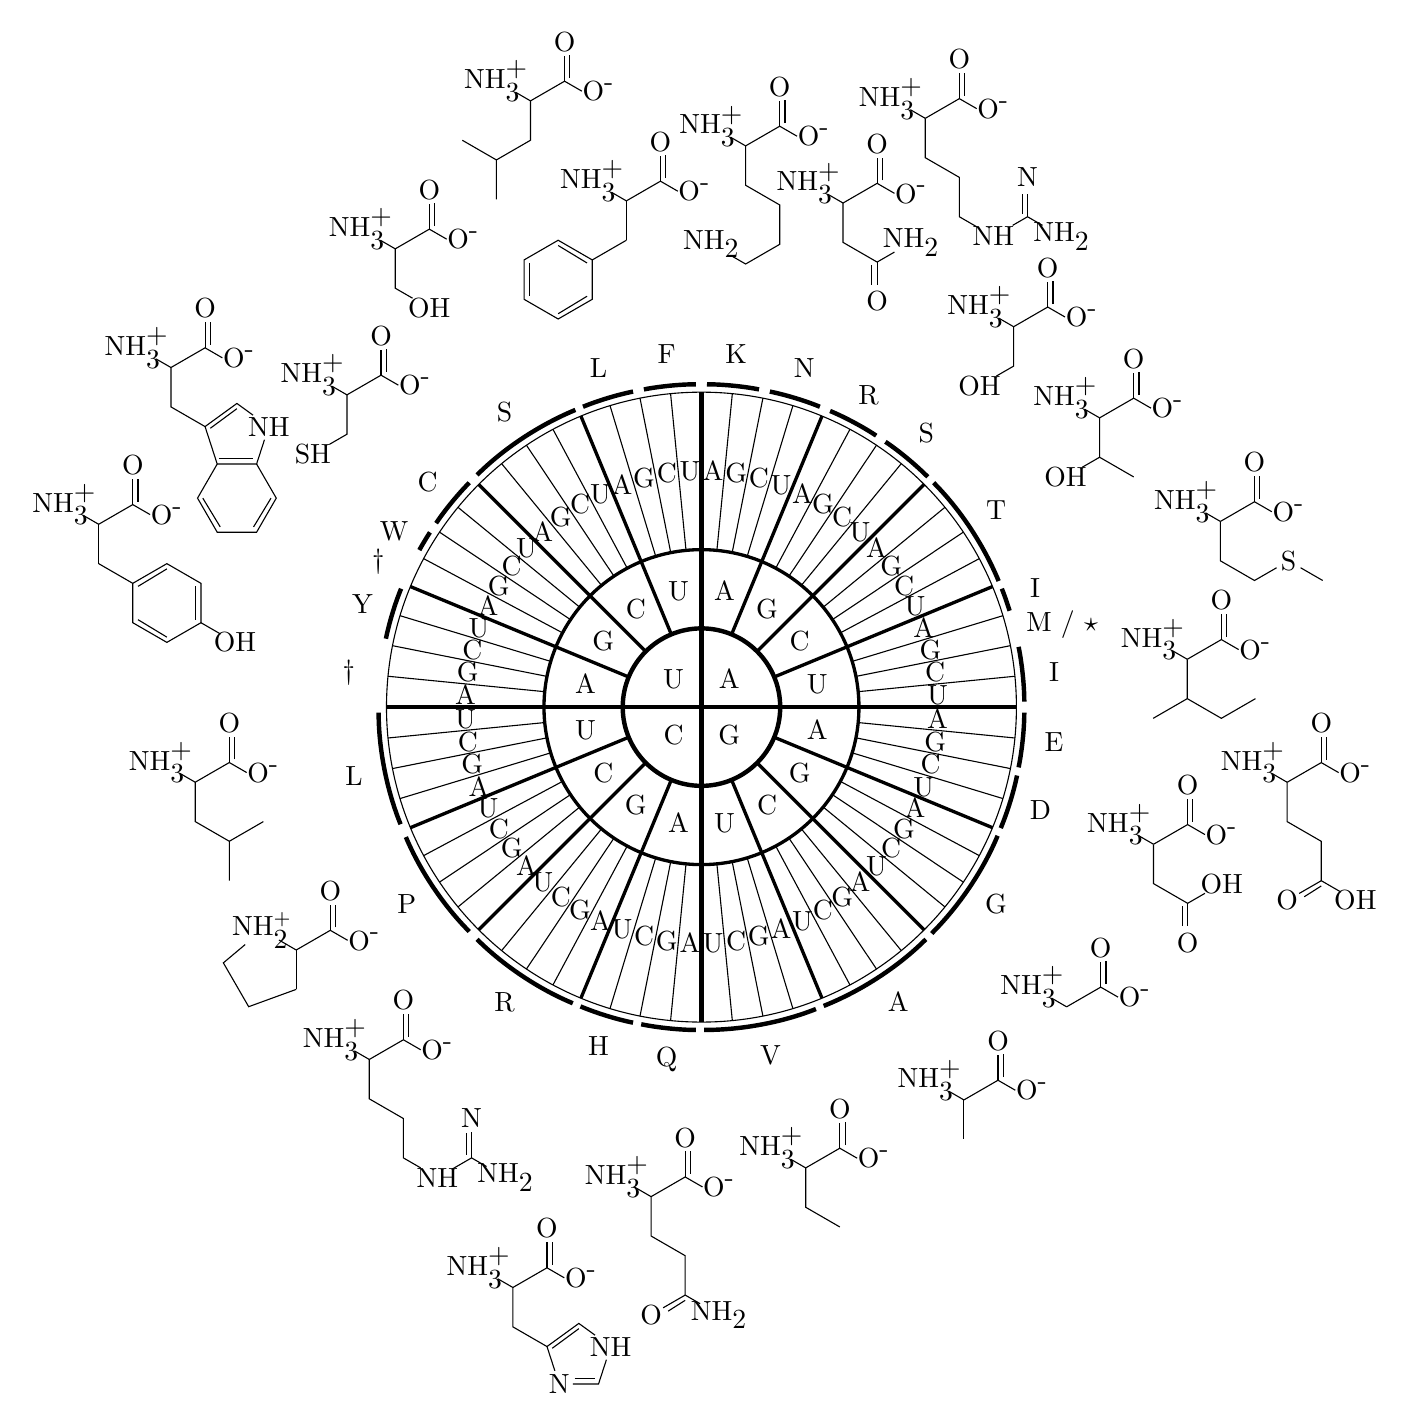
\begin{tikzpicture}
	\tikzstyle{every node}=[inner sep=1.7pt,anchor=center]
	%	to_x and from_x styles denote bonds terminating or starting in labeled nodes. x denotes the number of letters in the node label.
	\tikzstyle{to_1}=[shorten >=5pt]
	\tikzstyle{to_1i}=[shorten >=6pt]
	\tikzstyle{to_2}=[shorten >=7pt]
	\tikzstyle{to_3}=[shorten >=8pt]
	\tikzstyle{from_1}=[shorten <=5pt]
	\tikzstyle{from_1i}=[shorten <=6pt]
	\tikzstyle{from_2}=[shorten <=8pt]
	\begin{scope}
	\draw [ultra thick] circle(1cm);
	\draw [ultra thick] (0:4)--(180:4) (90:4)--(270:4);
	\foreach \a/\l in {45/A,135/G,225/C,315/U}{
		\node at (90-\a:0.5cm) {\l};
	}
	\draw [very thick] circle(2cm);
	\foreach \A in {90,0,270,180}{
		\foreach \a/\l in {22.5/A,45/G,67.5/C,90/U}{
			\draw [very thick] (\A+\a:1) -- (\A+\a:4);
			\node at (\A-\a+11.25:1.5) {\l};
		}
	}
	\draw circle(4cm) (0:4)--(180:4) (90:4)--(270:4);
	\foreach \A in {90,180,270,0}{
		\foreach \a in {0,22.5,45,67.5}{
			\foreach \i/\l in {5.625/A,11.25/G,16.875/C,22.5/U}{
				\draw (\A+\a+\i:2) -- (\A+\a+\i:4);
				\node at (\A-\a-\i+2.8125:3) {\l};
			}
		}
	}
	\end{scope}
	\begin{scope}[scale=0.5]	% Lysine
	\draw[ultra thick,shorten >=2pt,shorten <=2pt] (90:8.2)
	arc(90:90-2*5.625:8.2);
	\path (90-0.8*5.625:14.3) node (zero) {};
	\draw[to_2]  (zero.center)	-- ++(30:1) node (CO) {}  
	-- +(330:1) node [anchor=base] {O$^{\mbox{-}}$};
	\draw[to_1]  (CO.center) 	-- +(90:1) node (Od) {O};
	\draw[to_1i] (CO.30)		-- +(90:1);
	\draw[to_3]  (zero.center)	-- ++(150:1) node {NH$_{\mbox{3}}^{\mbox{+}}$};
	\draw[to_3]  (zero.center)	-- ++(270:1) node(Cb){}
	-- ++(330:1) node (Cc) {}
	-- ++(270:1) node (Cd) {}
	-- ++(210:1) node (Ce) {}
	-- ++(150:1) node (Cf) {NH$_{\mbox{2}}$};
	\end{scope}
	\begin{scope}[scale=0.5]	% Asparagine
	\draw[ultra thick,shorten >=2pt,shorten <=2pt] (90-2*5.625:8.2)
	arc(90-2*5.625:90-4*5.625:8.2);
	\path (90-3.5*3.625-3:13.3) node (zero) {};
	\draw[to_2]  (zero.center)	-- ++(30:1) node (CO) {} 
	-- +(330:1) node [anchor=base] {O$^{\mbox{-}}$};
	\draw[to_1]  (CO.center)	-- +(90:1) node (Od) {O};
	\draw[to_1i] (CO.30)		-- +(90:1);
	\draw[to_3]  (zero.center)	-- ++(150:1) node {NH$_{\mbox{3}}^{\mbox{+}}$};
	\draw[to_2]  (zero.center)	-- ++(270:1) node(Cb){}
	-- ++(330:1) node (Cc) {}
	-- +(30:1) node (Cd) {NH$_{\mbox{2}}$};
	\draw[to_1i] (Cc.center)	-- +(270:1) node (O) {};
	\draw[to_1]  (Cc.210)		-- (O.150);
	\path (O.center) node {O};
	\end{scope}
	\begin{scope}[scale=0.5]	% Arginine
	\draw[ultra thick,shorten >=2pt,shorten <=2pt] (90-22.5:8.2)
	arc(90-22.5:90-33.75:8.2);
	\path (90-3.7*5.625:16) node (zero) {};
	\draw[to_2]  (zero.center)	-- ++(30:1) node (CO) {}
	-- +(330:1) node [anchor=base] {O$^{\mbox{-}}$};
	\draw[to_1]  (CO.center)	-- +(90:1) node (Od) {O};
	\draw[to_1i] (CO.30)		-- +(90:1);
	\draw[to_3]  (zero.center)	-- ++(150:1) node {NH$_{\mbox{3}}^{\mbox{+}}$};
	\draw[to_2]  (zero.center)	-- ++(270:1) node(Cb){}
	-- ++(330:1) node (Cc) {}
	-- ++(270:1) node (Cd) {}
	-- ++(330:1) node (NH1) {NH};
	\draw[from_2,to_3]  (NH1.center)	-- ++(30:1) node (Ce) {}
	-- ++(330:1) node {NH$_{\mbox{2}}$};
	\draw[to_1i] (Ce.center)	-- ++(90:1) node (N2) {};
	\draw[to_1]  (Ce.150)		-- (N2.210);
	\path (N2) node {N};
	\end{scope}
	\begin{scope}[scale=0.5]	% Serine
	\draw[ultra thick,shorten >=1pt,shorten <=2pt] (90-22.5-2*5.625:8.2)
	arc(90-33.75:90-33.75-11.25:8.2);
	\path (90-7*5.625:12.5) node (zero) {};
	\draw[to_2]  (zero.center)	-- ++(30:1) node (CO) {}
	-- +(330:1) node [anchor=base] {O$^{\mbox{-}}$};
	\draw[to_1]  (CO.center)	-- +(90:1) node (Od) {O};
	\draw[to_1i] (CO.30)		-- +(90:1);
	\draw[to_3]  (zero.center)	-- ++(150:1) node {NH$_{\mbox{3}}^{\mbox{+}}$};
	\draw[to_2]  (zero.center)	-- ++(270:1) node(Cb){} -- ++(210:1) node (Cc) {OH};
	\end{scope}
	\begin{scope}[scale=0.5]	% Threonine
	\draw[ultra thick,shorten >=1pt,shorten <=2pt] (90-45:8.2)
	arc(90-45:90-67.5:8.2);
	\path (90-45-0.8*11.25:12.5) node (zero) {};
	\draw[to_2]  (zero.center)	-- ++(30:1) node (CO) {}
	-- +(330:1) node [anchor=base] {O$^{\mbox{-}}$};
	\draw[to_1]  (CO.center)	-- +(90:1) node (Od) {O};
	\draw[to_1i] (CO.30)		-- +(90:1);
	\draw[to_3]  (zero.center)	-- ++(150:1) node {NH$_{\mbox{3}}^{\mbox{+}}$};
	\draw[to_2]  (zero.center)	-- ++(270:1) node(Cb){}
	-- ++(330:1) node (Cc) {} (Cb.center)
	-- +(210:1) node {OH};
	\end{scope}
	\begin{scope}[scale=0.5]	% Methionine
	\draw[ultra thick,shorten >=1pt,shorten <=2pt] (90-67.5:8.2)
	arc(90-67.5:90-67.5-5.625:8.2);
	\path (90-67.5-0.5*5.625:14) node (zero) {};
	\draw[to_2]  (zero.center)	-- ++(30:1) node (CO) {}
	-- +(330:1) node [anchor=base] {O$^{\mbox{-}}$};
	\draw[to_1]  (CO.center)	-- +(90:1) node (Od) {O};
	\draw[to_1i] (CO.30)		-- +(90:1);
	\draw[to_3]  (zero.center)	-- ++(150:1) node {NH$_{\mbox{3}}^{\mbox{+}}$};
	\draw[to_1]  (zero.center)	-- ++(270:1) node(Cb){}
	-- ++(330:1) node (Cc) {}
	-- ++(30:1) node (Cd) {S};
	\draw[from_1] (Cd.center)	-- +(330:1);
	\end{scope}
	\begin{scope}[scale=0.5]	% Isoleucine
	\draw[ultra thick,shorten >=1pt,shorten <=2pt] (0:8.2)
	arc(0:11.25:8.2);
	\path (1.0*5.625:12.4) node (zero) {};
	\draw[to_2]  (zero.center)	-- ++(30:1) node (CO) {}
	-- +(330:1) node [anchor=base] {O$^{\mbox{-}}$};
	\draw[to_1]  (CO.center)	-- +(90:1) node (Od) {O};
	\draw[to_1i] (CO.30)		-- +(90:1);
	\draw[to_3]  (zero.center)	-- ++(150:1) node {NH$_{\mbox{3}}^{\mbox{+}}$};
	\draw	     (zero.center)	-- ++(270:1) node(Cb){}
	-- ++(330:1) node (Cc) {}
	-- +(30:1) node (Cd) {} (Cb.center)
	-- +(210:1) node (Ce) {};
	\end{scope}
	\begin{scope}[scale=0.5]	% Glutamic acid
	\draw[ultra thick,shorten >=1pt,shorten <=2pt] (0:8.2)
	arc(0:-11.25:8.2);
	\path (-1.3*5.625:15) node (zero) {};
	\draw[to_2]  (zero.center)	-- ++(30:1) node (CO) {}
	-- +(330:1) node [anchor=base] {O$^{\mbox{-}}$};
	\draw[to_1]  (CO.center)  	-- +(90:1) node (Od) {O};
	\draw[to_1i] (CO.30)  		-- +(90:1);
	\draw[to_3]  (zero.center) 	-- ++(150:1) node {NH$_{\mbox{3}}^{\mbox{+}}$};
	\draw[to_1i] (zero.center) 	-- ++(270:1) node(Cb){} 
	-- ++(330:1) node (Cc) {} 
	-- ++(270:1) node (Cd) {}
	-- ++(330:1) node (NH) {OH};
	\draw[to_1]  (Cd.center) 	-- +(210:1) node (O) {};
	\draw[to_1i] (Cd.270) 		-- (O.300);
	\path (O.center) node {O};
	\end{scope}
	\begin{scope}[scale=0.5]	% Aspartic acid
	\draw[ultra thick,shorten >=1pt,shorten <=2pt] (-11.25:8.2)
	arc(-11.25:-22.5:8.2);
	\path (-11.25-5.625:12) node (zero) {};
	\draw[to_2]  (zero.center)	-- ++(30:1) node (CO) {}
	-- +(330:1) node [anchor=base] {O$^{\mbox{-}}$};
	\draw[to_1]  (CO.center) 	-- +(90:1) node (Od) {O};
	\draw[to_1i] (CO.30)		-- +(90:1);
	\draw[to_3]  (zero.center)	-- ++(150:1) node {NH$_{\mbox{3}}^{\mbox{+}}$};
	\draw[to_2]  (zero.center)	-- ++(270:1) node(Cb){}
	-- ++(330:1) node (Cc) {}
	-- +(30:1) node (Cd) {OH};
	\draw[to_1i] (Cc.center)	-- +(270:1) node (O) {};
	\draw[to_1]  (Cc.210)		-- (O.150);
	\path (O.center) node {O};
	\end{scope}
	\begin{scope}[scale=0.5]	% Glycine
	\draw[ultra thick,shorten >=1pt,shorten <=2pt] (-22.5:8.2)
	arc(-22.5:-45:8.2);
	\path (-33.75-1*5.625:12) node (zero) {};
	\draw[to_2]  (zero.center)	-- ++(30:1) node (CO) {}
	-- +(330:1) node [anchor=base] {O$^{\mbox{-}}$};
	\draw[to_1]  (CO.center)	-- +(90:1) node (Od) {O};
	\draw[to_1i] (CO.30)		-- +(90:1);
	\draw[to_3]  (zero.center)	-- ++(150:1) node {NH$_{\mbox{3}}^{\mbox{+}}$};
	\end{scope}
	\begin{scope}[scale=0.5]	% Alanine
	\draw[ultra thick,shorten >=1pt,shorten <=2pt] (-45:8.2)
	arc(-45:-68.25:8.2);
	\path (-45-11.25:12) node (zero) {};
	\draw[to_2]  (zero.center)	-- ++(30:1) node (CO) {}
	-- +(330:1) node [anchor=base] {O$^{\mbox{-}}$};
	\draw[to_1]  (CO.center)	-- +(90:1) node (Od) {O};
	\draw[to_1i] (CO.30)		-- +(90:1);
	\draw[to_3]  (zero.center)	-- ++(150:1) node {NH$_{\mbox{3}}^{\mbox{+}}$};
	\draw	     (zero.center)	-- ++(270:1) node(Cb){};
	\end{scope}
	\begin{scope}[scale=0.5]	% Valine
	\draw[ultra thick,shorten >=1pt,shorten <=2pt] (-68.25:8.2)
	arc(-68.25:-90:8.2);
	\path (-68.25-0.8*11.25:12) node (zero) {};
	\draw[to_2]  (zero.center)	-- ++(30:1) node (CO) {}
	-- +(330:1) node [anchor=base] {O$^{\mbox{-}}$};
	\draw[to_1]  (CO.center)	-- +(90:1) node (Od) {O};
	\draw[to_1i] (CO.30)		-- +(90:1);
	\draw[to_3]  (zero.center)	-- ++(150:1) node {NH$_{\mbox{3}}^{\mbox{+}}$};
	\draw (zero.center)		-- ++(270:1) node(Cb){}
	-- ++(330:1) node (Cc) {};
	\end{scope}
	\begin{scope}[scale=0.5]	% Glutamine
	\draw[ultra thick,shorten >=1pt,shorten <=2pt] (-90:8.2)
	arc(-90:-101.25:8.2);
	\path (-90.25-5.625:12.5) node (zero) {};
	\draw[to_2]  (zero.center)	-- ++(30:1) node (CO) {}
	-- +(330:1) node [anchor=base] {O$^{\mbox{-}}$};
	\draw[to_1]  (CO.center)	-- +(90:1) node (Od) {O};
	\draw[to_1i] (CO.30)		-- +(90:1);
	\draw[to_2]  (zero.center)	-- ++(150:1) node {NH$_{\mbox{3}}^{\mbox{+}}$};
	\draw[to_3]  (zero.center)	-- ++(270:1) node(Cb){}
	-- ++(330:1) node (Cc) {}
	-- ++(270:1) node (Cd) {}
	-- ++(330:1) node (NH) {NH$_{\mbox{2}}$};
	\draw[to_1]  (Cd.center)	-- +(210:1) node (O) {};
	\draw[to_1i] (Cd.270)		-- (O.300);
	\path (O.center) node {O};
	\end{scope}
	\begin{scope}[scale=0.5]	% Histidine
	\draw[ultra thick,shorten >=1pt,shorten <=2pt] (-101.25:8.2)
	arc(-101.25:-101.25-11.25:8.2);
	\path (-101.25-1.2*5.625:15.5) node (zero) {};
	\draw[to_2]  (zero.center)	-- ++(30:1) node (CO) {}
	-- +(330:1) node [anchor=base] {O$^{\mbox{-}}$};
	\draw[to_1]  (CO.center)	-- +(90:1) node (Od) {O};
	\draw[to_1i] (CO.30)		-- +(90:1);
	\draw[to_3]  (zero.center)	-- ++(150:1) node {NH$_{\mbox{3}}^{\mbox{+}}$};
	\draw        (zero.center)	-- ++(270:1) node(Cb){}
	-- ++(330:1) node(Cc){};
	\draw[to_2]  (Cc.center)	-- ++(108-1*72:1) node (Cd) {}
	-- ++(108-2*72:1) node (Ce) {NH};
	\draw[from_1,to_1] (Ce.center)	-- ++(108-3*72:1) node (Cf) {}
	-- ++(108-4*72:1) node (Cg) {};
	\draw[from_1] (Cg.center)	-- (Cc.center);
	\draw         (Cc.198+2*72)	-- (Cd.198+1*72);
	\draw[from_1] (Cg.72)		-- (Cf.198+4*72);
	\draw (Cg.center) node {N};
	\end{scope}
	\begin{scope}[scale=0.5]	% Arginine
	\draw[ultra thick,shorten >=2pt,shorten <=2pt] (-90-22.5:8.2)
	arc(-90-22.5:-90-45:8.2);
	\path (-90-7.7*5.625:12.3) node (zero) {};
	\draw[to_2]  (zero.center)	-- ++(30:1) node (CO) {}
	-- +(330:1) node [anchor=base] {O$^{\mbox{-}}$};
	\draw[to_1]  (CO.center)	-- +(90:1) node (Od) {O};
	\draw[to_1i] (CO.30)		-- +(90:1);
	\draw[to_3]  (zero.center)	-- ++(150:1) node {NH$_{\mbox{3}}^{\mbox{+}}$};
	\draw[to_2]  (zero.center)	-- ++(270:1) node(Cb){}
	-- ++(330:1) node (Cc) {}
	-- ++(270:1) node (Cd) {}
	-- ++(330:1) node (NH1) {NH};
	\draw[from_1i,to_3] (NH1.center)-- ++(30:1) node (Ce) {}
	-- ++(330:1) node {NH$_{\mbox{2}}$};
	\draw[to_1]  (Ce.center)	-- ++(90:1) node (N2) {};
	\draw[shorten >=4pt] (Ce.150)	-- (N2.210);
	\path (N2) node {N};
	\end{scope}
	\begin{scope}[scale=0.5]	% Proline
	\draw[ultra thick,shorten >=2pt,shorten <=2pt] (-90-45:8.2)
	arc(-90-45:-90-45-22.25:8.2);
	\path (-90-10.5*5.625:12) node (zero) {};
	\draw[to_2]  (zero.center)	-- ++(30:1) node (CO) {}
	-- +(330:1) node [anchor=base] {O$^{\mbox{-}}$};
	\draw[to_1]  (CO.center)	-- +(90:1) node (Od) {O};
	\draw[to_1i] (CO.30)		-- +(90:1);
	\draw[to_2]  (zero.center)	-- ++(150:1) node (nh) {NH$_{\mbox{2}}^+$};
	\draw        (zero.center)	-- ++(270:1) node(Cb){};
	\path        (Cb.center)	-- +(150:1) node (x) {};
	\path        (x.center)  	+(170:1) node (Cd) {};
	\path        (x.center)  	+(250:1) node (Cc) {};
	\draw[to_3]  (Cb.center)	-- (Cc.center)
	-- (Cd.center)
	-- (nh.center);
	\end{scope}
	\begin{scope}[scale=0.5]	% Leucine
	\draw[ultra thick,shorten >=2pt,shorten <=2pt] (180:8.2)
	arc(180:180+22.25:8.2);
	\path (-90-14.5*5.625:13) node (zero) {};
	\draw[to_2]  (zero.center)	-- ++(30:1) node (CO) {}
	-- +(330:1) node [anchor=base] {O$^{\mbox{-}}$};
	\draw[to_1]  (CO.center)	-- +(90:1) node (Od) {O};
	\draw[to_1i] (CO.30)		-- +(90:1);
	\draw[to_3]  (zero.center)	-- ++(150:1) node {NH$_{\mbox{3}}^{\mbox{+}}$};
	\draw (zero.center)		-- ++(270:1) node(Cb){}
	-- ++(330:1) node (Cc) {}
	-- +(30:1) node (Cd) {} (Cc.center)
	-- +(270:1) node (Ce) {};
	\end{scope}
	\begin{scope}[scale=0.5]	% Tyrosine
	\draw[ultra thick,shorten >=2pt,shorten <=2pt] (180-11.25:8.2)
	arc(180-11.25:180-22.5:8.2);
	\path (180-3*5.625:16) node (zero) {};
	\draw[to_2]  (zero.center)	-- ++(30:1) node (CO) {}
	-- +(330:1) node [anchor=base] {O$^{\mbox{-}}$};
	\draw[to_1]  (CO.center)	-- +(90:1) node (Od) {O};
	\draw[to_1i] (CO.30)		-- +(90:1);
	\draw[to_3]  (zero.center)	-- ++(150:1) node {NH$_{\mbox{3}}^{\mbox{+}}$};
	\draw 	     (zero.center)	-- ++(270:1) node(Cb){};
	\draw	     (Cb.center)	-- ++(330:1) node (Cc) {}
	-- ++(30:1) node (Cd) {}
	-- ++(330:1) node (Ce) {}
	-- ++(270:1) node (Cf) {}
	-- ++(210:1) node (Cg) {}
	-- ++(150:1) node (Ch) {}
	-- ++(90:1);
	\draw        (Cc.330)		-- (Cd.270);
	\draw        (Ce.210)		-- (Cf.150);
	\draw        (Cg.90)		-- (Ch.30);
	\draw[to_1i] (Cf.center)	-- +(330:1) node (OH) {OH};
	\end{scope}
	\begin{scope}[scale=0.5]	% Tryptophane
	\draw[ultra thick,shorten >=2pt,shorten <=2pt] (180-22.5-5.625:8.2)
	arc(180-22.5-5.625:180-22.5-11.25:8.2);
	\path (180-22.5-1.8*5.625:16) node (zero) {};
	\draw[to_2]  (zero.center)	-- ++(30:1) node (CO) {}
	-- +(330:1) node [anchor=base] {O$^{\mbox{-}}$};
	\draw[to_1]  (CO.center)	-- +(90:1) node (Od) {O};
	\draw[to_1i] (CO.30)		-- +(90:1);
	\draw[to_3]  (zero.center)	-- ++(150:1) node {NH$_{\mbox{3}}^{\mbox{+}}$};
	\draw 	     (zero.center)	-- ++(270:1) node(Cb){}
	-- ++(330:1) node(Cc){};
	\draw[to_2]  (Cc.center)	-- ++(108-1*72:1) node (Cd) {}
	-- ++(108-2*72:1) node (Ce) {NH};
	\draw[from_1](Ce.center)	-- ++(108-3*72:1) node (Cf) {}
	-- ++(108-4*72:1) node (Cg) {};
	\draw 	     (Cg.center)	-- (Cc.center);
	\draw        (Cc.198+2*72)	-- (Cd.198+1*72);
	\draw 	     (Cg.72)		-- (Cf.198+4*72);
	\draw	     (Cg.center)	-- ++(240:1) node (Ch) {}
	-- ++(300:1) node (Ci) {}
	-- ++(0:1) node (Cj) {}
	-- ++(60:1) node (Ck) {}
	-- ++(120:1) node (Cl) {};
	\draw	     (Ch.0)		-- (Ci.60);
	\draw	     (Cj.120)		-- (Ck.180);
	\end{scope}
	\begin{scope}[scale=0.5]	% Cysteine
	\draw[ultra thick,shorten >=2pt,shorten <=2pt] (180-45+11.25:8.2)
	arc(180-45+11.25:180-45:8.2);
	\path (180-45+11.25-1*7.625:12) node (zero) {};
	\draw[to_2]  (zero.center)	-- ++(30:1) node (CO) {}
	-- +(330:1) node [anchor=base] {O$^{\mbox{-}}$};
	\draw[to_1]  (CO.center)	-- +(90:1) node (Od) {O};
	\draw[to_1i] (CO.30)		-- +(90:1);
	\draw[to_3]  (zero.center)	-- ++(150:1) node {NH$_{\mbox{3}}^{\mbox{+}}$};
	\draw[to_2]  (zero.center)	-- ++(270:1) node(Cb){}
	-- ++(210:1) node (Cc) {SH};
	\end{scope}
	\begin{scope}[scale=0.5]	% Serine
	\draw[ultra thick,shorten >=1pt,shorten <=2pt] (90+45:8.2)
	arc(90+45:90+45-22.5:8.2);
	\path (90+45-11.25+0*5.625:14) node (zero) {};
	\draw[to_2]  (zero.center)	-- ++(30:1) node (CO) {}
	-- +(330:1) node [anchor=base] {O$^{\mbox{-}}$};
	\draw[to_1]  (CO.center)	-- +(90:1) node (Od) {O};
	\draw[to_1i] (CO.30)		-- +(90:1);
	\draw[to_3]  (zero.center)	-- ++(150:1) node {NH$_{\mbox{3}}^{\mbox{+}}$};
	\draw[to_2]  (zero.center)	-- ++(270:1) node(Cb){}
	-- ++(330:1) node (Cc) {OH};
	\end{scope}
	\begin{scope}[scale=0.5]	% Leucine
	\draw[ultra thick,shorten >=2pt,shorten <=2pt] (90+22.5:8.2)
	arc(90+22.5:90+11.25:8.2);
	\path (90+22.5-1.2*5.625:16) node (zero) {};
	\draw[to_2]  (zero.center)	-- ++(30:1) node (CO) {}
	-- +(330:1) node [anchor=base] {O$^{\mbox{-}}$};
	\draw[to_1]  (CO.center)	-- +(90:1) node (Od) {O};
	\draw[to_1i] (CO.30)		-- +(90:1);
	\draw[to_3]  (zero.center)	-- ++(150:1) node {NH$_{\mbox{3}}^{\mbox{+}}$};
	\draw 	     (zero.center)	-- ++(270:1) node(Cb){}
	-- ++(210:1) node (Cc) {}
	-- +(150:1) node (Cd) {} (Cc.center)
	-- +(270:1) node (Ce) {};
	\end{scope}
	\begin{scope}[scale=0.5]	% Phenylalanine
	\draw[ultra thick,shorten >=2pt,shorten <=2pt] (90+11.25:8.2)
	arc(90+11.25:90:8.2);
	\path (90+1.5*5.625:13) node (zero) {};
	\draw[to_2]  (zero.center)	-- ++(30:1) node (CO) {}
	-- +(330:1) node [anchor=base] {O$^{\mbox{-}}$};
	\draw[to_1]  (CO.center)	-- +(90:1) node (Od) {O};
	\draw[to_1i] (CO.30)		-- +(90:1);
	\draw[to_3]  (zero.center)	-- ++(150:1) node {NH$_{\mbox{3}}^{\mbox{+}}$};
	\draw	     (zero.center)	-- ++(270:1) node(Cb){};
	\draw	     (Cb.center)	-- ++(210:1) node (Cc) {}
	-- ++(150:1) node (Cd) {}
	-- ++(210:1) node (Ce) {}
	-- ++(270:1) node (Cf) {}
	-- ++(330:1) node (Cg) {}
	-- ++(30:1) node (Ch) {}
	-- ++(90:1);
	\draw	     (Cc.210)		-- (Cd.270);
	\draw	     (Ce.330)		-- (Cf.30);
	\draw	     (Cg.90)		-- (Ch.150);
	\end{scope}
	\node at (90-1*5.625:4.5) {K};
	\node at (90-3*5.625:4.5) {N};
	\node at (90-5*5.625:4.5) {R};
	\node at (90-7*5.625:4.5) {S};
	\node at (90-10*5.625:4.5) {T};
	\node at (90-12.5*5.625:4.5) {I};
	\node at (90-13.7*5.625:4.7) {M / $\star$};
	\node at (90-15*5.625:4.5) {I};
	\node at (90-17*5.625:4.5) {E};
	\node at (90-19*5.625:4.5) {D};
	\node at (90-22*5.625:4.5) {G};
	\node at (90-26*5.625:4.5) {A};
	\node at (90-30*5.625:4.5) {V};
	\node at (90-33*5.625:4.5) {Q};
	\node at (90-35*5.625:4.5) {H};
	\node at (90-38*5.625:4.5) {R};
	\node at (90-42*5.625:4.5) {P};
	\node at (90-46*5.625:4.5) {L};
	\node at (90-49*5.625:4.5) {$\dagger$};
	\node at (90-51*5.625:4.5) {Y};
	\node at (90-52.3*5.625:4.5) {$\dagger$};
	\node at (90-53.3*5.625:4.5) {W};
	\node at (90-55*5.625:4.5) {C};
	\node at (90-58*5.625:4.5) {S};
	\node at (90-61*5.625:4.5) {L};
	\node at (90-63*5.625:4.5) {F};
	\end{tikzpicture}
\end{center}

\normalfont

\section{Ví dụ 2 - câu lệnh vẽ cây tìm kiếm đệ quy}
\ovalbox{
	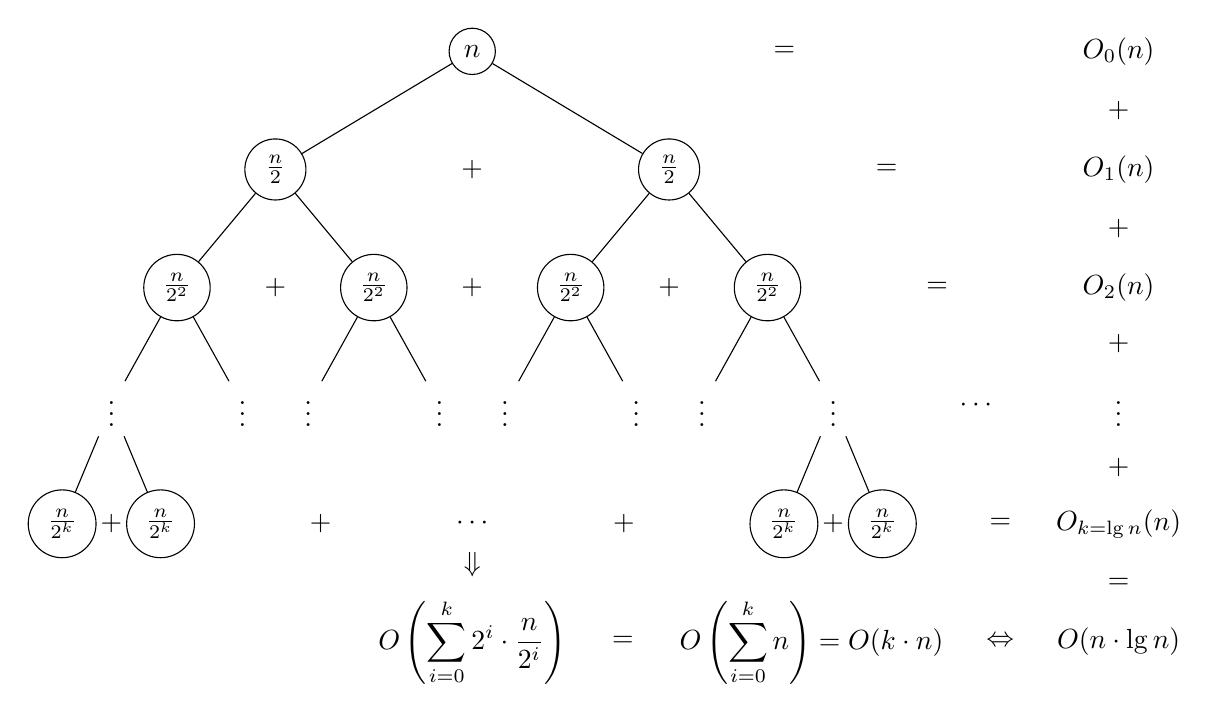
\begin{tikzpicture}[level/.style={sibling distance=50mm/#1}]
	\node [circle,draw] (z){$n$}
	child {node [circle,draw] (a) {$\frac{n}{2}$}
		child {node [circle,draw] (b) {$\frac{n}{2^2}$}
			child {node {$\vdots$}
				child {node [circle,draw] (d) {$\frac{n}{2^k}$}}
				child {node [circle,draw] (e) {$\frac{n}{2^k}$}}
			} 
			child {node {$\vdots$}}
		}
		child {node [circle,draw] (g) {$\frac{n}{2^2}$}
			child {node {$\vdots$}}
			child {node {$\vdots$}}
		}
	}
	child {node [circle,draw] (j) {$\frac{n}{2}$}
		child {node [circle,draw] (k) {$\frac{n}{2^2}$}
			child {node {$\vdots$}}
			child {node {$\vdots$}}
		}
		child {node [circle,draw] (l) {$\frac{n}{2^2}$}
			child {node {$\vdots$}}
			child {node (c){$\vdots$}
				child {node [circle,draw] (o) {$\frac{n}{2^k}$}}
				child {node [circle,draw] (p) {$\frac{n}{2^k}$}
					child [grow=right] {node (q) {$=$} edge from parent[draw=none]
						child [grow=right] {node (q) {$O_{k = \lg n}(n)$} edge from parent[draw=none]
							child [grow=up] {node (r) {$\vdots$} edge from parent[draw=none]
								child [grow=up] {node (s) {$O_2(n)$} edge from parent[draw=none]
									child [grow=up] {node (t) {$O_1(n)$} edge from parent[draw=none]
										child [grow=up] {node (u) {$O_0(n)$} edge from parent[draw=none]}
									}
								}
							}
							child [grow=down] {node (v) {$O(n \cdot \lg n)$}edge from parent[draw=none]}
						}
					}
				}
			}
		}
	};
	\path (a) -- (j) node [midway] {+};
	\path (b) -- (g) node [midway] {+};
	\path (k) -- (l) node [midway] {+};
	\path (k) -- (g) node [midway] {+};
	\path (d) -- (e) node [midway] {+};
	\path (o) -- (p) node [midway] {+};
	\path (o) -- (e) node (x) [midway] {$\cdots$}
	child [grow=down] {
		node (y) {$O\left(\displaystyle\sum_{i = 0}^k 2^i \cdot \frac{n}{2^i}\right)$}
		edge from parent[draw=none]
	};
	\path (q) -- (r) node [midway] {+};
	\path (s) -- (r) node [midway] {+};
	\path (s) -- (t) node [midway] {+};
	\path (s) -- (l) node [midway] {=};
	\path (t) -- (u) node [midway] {+};
	\path (z) -- (u) node [midway] {=};
	\path (j) -- (t) node [midway] {=};
	\path (y) -- (x) node [midway] {$\Downarrow$};
	\path (v) -- (y)
	node (w) [midway] {$O\left(\displaystyle\sum_{i = 0}^k n\right) = O(k \cdot n)$};
	\path (q) -- (v) node [midway] {=};
	\path (e) -- (x) node [midway] {+};
	\path (o) -- (x) node [midway] {+};
	\path (y) -- (w) node [midway] {$=$};
	\path (v) -- (w) node [midway] {$\Leftrightarrow$};
	\path (r) -- (c) node [midway] {$\cdots$};
\end{tikzpicture}}

%\subsection{title}
\section{Ví dụ 3 - vẽ lưới và tọa độ cực}	
\begin{center}

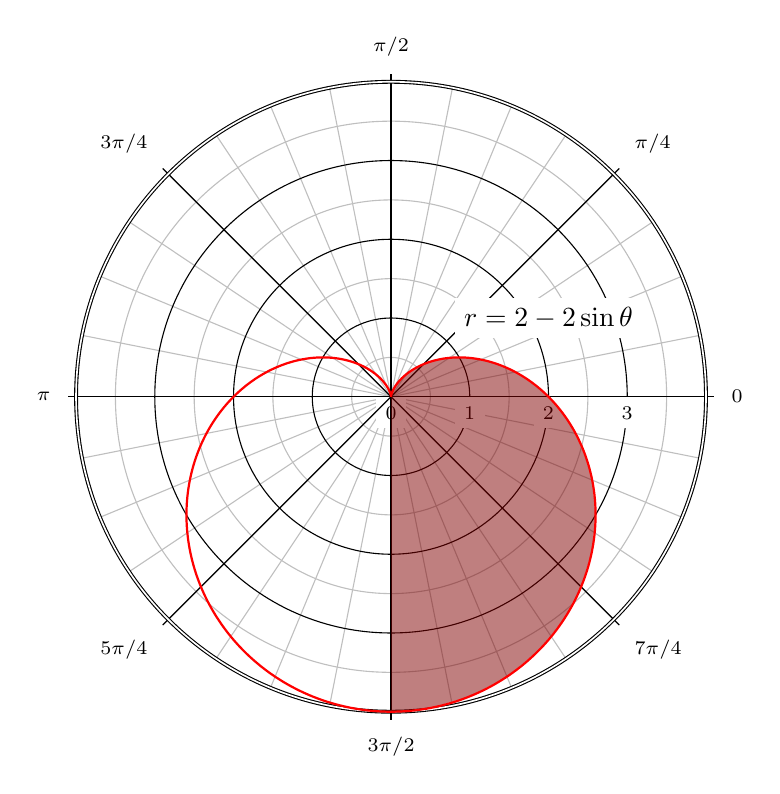
\begin{tikzpicture}[>=latex]
\foreach \ang in {0,...,31} {
	\draw [lightgray] (0,0) -- (\ang * 180 / 16:4);
}

% Concentric circles and radius labels
\foreach \s in {0, 1, 2, 3} {
	\draw [lightgray] (0,0) circle (\s + 0.5);
	\draw (0,0) circle (\s);
	\node [fill=white] at (\s, 0) [below] {\scriptsize $\s$};
}

% Add the labels at multiples of pi/4
\foreach \ang/\lab/\dir in {
	0/0/right,
	1/{\pi/4}/{above right},
	2/{\pi/2}/above,
	3/{3\pi/4}/{above left},
	4/{\pi}/left,
	5/{5\pi/4}/{below left},
	7/{7\pi/4}/{below right},
	6/{3\pi/2}/below} {
	\draw (0,0) -- (\ang * 180 / 4:4.1);
	\node [fill=white] at (\ang * 180 / 4:4.2) [\dir] {\scriptsize $\lab$};
}

% The double-lined circle around the whole diagram
\draw [style=double] (0,0) circle (4);

\fill [fill=red!50!black, opacity=0.5] plot [domain=-pi/2:pi/2]
(xy polar cs:angle=\x r, radius= {2-2*sin(\x r)});
\draw [thick, color=red, domain=0:2*pi, samples=200, smooth]
plot (xy polar cs:angle=\x r, radius={2-2*sin(\x r)});
\node [fill=white] at (2,1) {$r=2-2\sin\theta$};

\end{tikzpicture} 
\end{center}
%\includepdf[pages=-,pagecommand={}]{BienBanThuNghiem.pdf}

\usetikzlibrary{arrows,automata}
\usetikzlibrary{positioning}


\tikzset{
	state/.style={
		rectangle,
		rounded corners,
		draw=black, very thick,
		minimum height=2em,
		inner sep=2pt,
		text centered,
	},
}


\section{Ví dụ 4 - câu lệnh vẽ sơ đồ nguyên lý}
\usetikzlibrary{decorations.pathmorphing} % for snake lines
\usetikzlibrary{matrix} % for block alignment
\usetikzlibrary{arrows} % for arrow heads
\usetikzlibrary{calc} % for manimulation of coordinates

% TikZ styles for drawing
\tikzstyle{block} = [draw,rectangle,thick,minimum height=2em,minimum width=2em]
\tikzstyle{sum} = [draw,circle,inner sep=0mm,minimum size=2mm]
\tikzstyle{connector} = [->,thick]
\tikzstyle{line} = [thick]
\tikzstyle{branch} = [circle,inner sep=0pt,minimum size=1mm,fill=black,draw=black]
\tikzstyle{guide} = []
\tikzstyle{snakeline} = [connector, decorate, decoration={pre length=0.2cm,
	post length=0.2cm, snake, amplitude=.4mm,
	segment length=2mm},thick, magenta, ->]

\renewcommand{\vec}[1]{\ensuremath{\boldsymbol{#1}}} % bold vectors
\def \myneq {\skew{-2}\not =} % \neq alone skews the dash	
	
\begin{center}
	
\begin{tikzpicture}[scale=1, auto, >=stealth']
	\small
	% node placement with matrix library: 5x4 array
	\matrix[ampersand replacement=\&, row sep=0.2cm, column sep=0.4cm] {
		%
		\node[block] (F1) {$\vec{u}_i = F_i(\{\widetilde{\vec{x}}_j\}_{j=1}^N)$}; \&
		\node[branch] (u1) {}; \&
		\&
		\node[block] (f1) {$\begin{matrix}
			\dot{\vec{x}}_i =
			f_i(\vec{x}_i,
			\textcolor{red}{\{\widetilde{\vec{x}}_j\}_{j \myneq i}},
			\vec{u}_i,
			t)\\
			\vec{y}_i =
			g_i(\vec{x}_i,
			\textcolor{blue}{\{\widetilde{\vec{x}}_j\}_{j \myneq i}},
			t)
			\end{matrix}$}; \& \\
		
		\&
		\&
		\&
		\node[block] (L1) {$\vec{e}_i(\vec{y}_i - \widetilde{\vec{y}}_i)$};\&
		\node [sum] (e1) {}; \\
		
		\&
		\&
		\node[sum] (v1) {}; \&
		\node[block] (o1) {$\begin{matrix}
			\dot{\widetilde{\vec{x}}}_i =
			\widetilde{f}_i(\widetilde{\vec{x}}_i,
			\textcolor{red}{\{\widetilde{\vec{x}}_j\}_{j \myneq i}},
			\vec{v}_i, t)\\
			\widetilde{\vec{y}}_i =
			g_i(\widetilde{\vec{x}}_i,
			\textcolor{blue}{\{\widetilde{\vec{x}}_j\}_{j \myneq i}},
			t)
			\end{matrix}$};
		\&
		\\
		\node[guide] (i1) {}; \& \& \& \& \\
	};
	
	% now link the nodes
	\draw [line] (F1) -- (u1);
	\draw [connector] (u1) -- node {$u_i$} (f1);
	\draw [connector] (f1) -| node[near end] {$\vec{y}_i$} (e1);
	\draw [connector] (e1) -- (L1);
	\draw [connector] (L1) -| (v1);
	\draw [connector] (v1) -- node {$\vec{v}_i$} (o1);
	\draw [connector] (u1) |- (v1);
	\draw [connector] (o1) -| node[pos=0.96] {$-$} node [near end, swap]
	{$\widetilde{\vec{y}}_i$} (e1);
	\draw [connector] (o1.south) -- ++(0,-.5cm) -| node [near start]
	{$\widetilde{\vec{x}}_i$} ($(F1.south) + (0.4cm, 0em)$);
	
	% draw the snake lines with offset (using the calc library)
	\draw [snakeline] ($(i1) - (0.4cm, -1cm)$) -- node
	{$\{\widetilde{\vec{x}}_j\}_{j \myneq i}$} ($(F1.south) - (0.4cm, 0em)$);
	
	\draw [snakeline, swap] ($(v1.east) - (1.0cm, 0.4cm)$) -- node
	{$\{\widetilde{\vec{x}}_j\}_{j \myneq i}$} ($(o1.west) - (0cm, 0.4cm)$);
	
	\draw [snakeline, swap] ($(u1.east) + (0.1cm, -0.4cm)$) -- node
	{$\{\widetilde{\vec{x}}_j\}_{j \myneq i}$} ($(f1.west) - (0cm, 0.4cm)$);
	
\end{tikzpicture}	
\end{center}
	
\section{ví dụ 5 - câu lệnh vẽ máy Oscilloscope}
\def\scl{0.6}%scaling factor of the picture

\begin{center}
\begin{tikzpicture}[
scale=\scl,
controlpanels/.style={yellow!30!brown!20!,rounded corners,draw=black,thick},
screen/.style={green!50!black!60!,draw=black,thick},
trace/.style={green!60!yellow!40!, ultra thick},
smallbutton/.style={white,draw=black, thick},
axes/.style={thick}]
\fill[green!30!blue!30!,rounded corners,draw=black,thick](0,0)
rectangle (27.75,13.25);
\fill[fill=black!40!,draw=black,thick,rounded corners](0.25,0.25)
rectangle (27.5,13.00);
% Screen, centered around the origin then shifted for easy plotting
\begin{scope}[xshift=7cm,yshift=8cm,samples=150]
\fill[black!60!,rounded corners,draw=black,thick](-5.3,-4.3)
rectangle (5.3,4.3);
\fill[screen] (-5.0,-4.0) rectangle (5.0,4.0);
\draw[trace] plot(\x,{1+2.4*sin((2.5*\x +1) r)}); % r for radians...
\draw[trace] plot(\x,{-1+1.25*sin((0.75*\x) r});
\draw[thin] (-5.0,-4.0) grid (5.0,4.0);
\draw[axes] (-5,0)--(5,0); % Time axis
\draw[axes] (0,-4)--(0,4);
\foreach \i in {-4.8,-4.6,...,4.8} \draw (\i,-0.1)--(\i,0.1);
\foreach \i in {-3.8,-3.6,...,3.8} \draw (-0.1,\i)--(0.1,\i);
\end{scope}
% Feet
\fill[black!70!,rounded corners,xshift=2cm] (0,-.5) rectangle (2,0);
\fill[black!70!,rounded corners,xshift=23.75cm] (0,-.5) rectangle (2,0);
% Lower left panel
\fill[controlpanels] (0.6,0.5) rectangle (13.5,3.0);
\path (0.8,0.9) node[scale=\scl,right]{$\mathbf{TeXtronics\,1 - v.1.01}$};
% Lower right panel
\fill[controlpanels] (13.7,0.5) rectangle (27.1,6.2);
%Channels
% CH I
\draw[thick] (14.8,1.5) circle (0.7cm);
\fill[gray,draw=black,thick] (14.8,1.5) circle (0.5cm);
\fill[white,draw=black,thick] (14.8,1.5) circle (0.3cm);
\node[scale={1.5*\scl}] at (14.8,2.5) {CH I};
\draw[thick] (16.2,1.5) circle (0.4cm);
\fill[black!60!] (16.2,1.5) circle (0.3cm);
\draw[thick] (16.6,1.5) --(17,1.5)--(17,1.0);
\draw[thick] (16.7,1.0)--(17.3,1.0);
\draw[thick] (16.8,0.85)--(17.2,0.85);
\draw[thick] (16.9,0.70)--(17.1,0.70);
\draw[thick] (26.0,1.5) circle (0.7cm);
% CH II
\fill[gray,draw=black,thick] (26,1.5) circle (0.5cm);
\fill[white,draw=black,thick] (26,1.5) circle (0.3cm);
\node[scale={1.5*\scl}] at (26,2.5) {CH II};
\draw[thick] (24.6,1.5) circle (0.4cm);
\fill[black!60!] (24.6,1.5) circle (0.3cm);
\draw[thick] (24.2,1.5) --(23.7,1.5)--(23.7,1.0);
\draw[thick] (23.4,1.0)--(24.0,1.0);
\draw[thick] (23.5,0.85)--(23.9,0.85);
\draw[thick] (23.6,0.70)--(23.8,0.70);
\draw[thick] (26.0,1.5) circle (0.7cm);
% Y-pos
\fill[smallbutton] (14.8,4.9) circle (0.3cm);
\node[scale={\scl}] at (14.8,5.5) {Y-pos I};
\fill[smallbutton] (26.0,4.9) circle (0.3cm);
\node[scale={\scl}] at (26.0,5.5) {Y-pos II};
% Volt/div the foreach loop draws the two buttons
\foreach \i / \b in {18/75,22.5/345}{
	%Second parameter of the loop is the angle of the index mark 
	\begin{scope}[xshift=\i cm,yshift=3.8cm,scale=0.85]
	\node[scale=\scl] at (0,2.3) {Volts/Div};
	\node[scale=\scl,black] at (-1,-2.4) {V};
	\node[scale=\scl,blue]  at (1,-2.4) {mV};
	\clip[rounded corners] (-2,-2) rectangle (2,2);
	\fill[black!30!,rounded corners,draw=black,thick] (-2,-2)
	rectangle (2,2);
	\fill[blue!50!black!20!,draw=black,thick]
	(30:1.1)--(30:3)--(3,-3)--(-90:3)--(-90:1.1) arc (-90:30:1.1);
	\draw[very thick,rounded corners](-2,-2) rectangle (2,2);
	\draw[thick] (0,0) circle (1.0);
	\foreach \i in {0,30,...,330}
	\draw[thick] (\i:1.2)--(\i:2.5);
	\foreach \i/\j in {15/50,45/.1,75/.2,105/.5,135/1,165/2,195/5,225/10,
		255/20,285/5,315/10,345/20} \node[scale=\scl,black] at (\i:1.7) {\j};
	\fill[blue!30!black!60!,draw=black,thick] (0,0) circle (0.8cm);
	% Here you set the right Volts/Div button
	\draw[ultra thick,red] (\b:0.3)--(\b:1.2);
	\end{scope}}
% Upper right panel
\fill[controlpanels] (13.7,6.5) rectangle (27.1,12.75);
%On-Off button
\draw[rounded corners,thick,blue] (13.9,10.5) rectangle (15.9,12.5);
\fill[fill=red,draw=black,thick,rounded corners] (14.4,10.8) rectangle (15.3,11.2);
\node[scale=\scl] at (14.8,12) {\textbf{Power}};
\node[scale=\scl] at (14.8,11.5) {\textbf{On/Off}};
% Focus-Intensity buttons
\draw[rounded corners,thick,blue] (13.9,7.0) rectangle (15.9,10.0);
\fill[smallbutton] (14.9,7.5) circle (0.3cm);
\node[scale=\scl] at (14.9,8.2) {\textbf{Focus}};
\fill[smallbutton] (14.9,9) circle (0.3cm);
\node[scale=\scl] at (14.9,9.6) {\textbf{Intens}};
% X-pos
\fill[smallbutton] (24.5,9.9) circle (0.3cm);
\node[scale={\scl}] at (24.5,10.5) {X-pos};
% Time/Div
\begin{scope}[xshift=21cm,yshift=9.5cm,scale=1]
\node[scale={1.25*\scl}]  at (0,2.4) {Time/Div};
\clip[rounded corners] (-2.2,-2) rectangle (2.2,2);
\fill[black!30!,rounded corners,draw=black,thick] (-2.2,-2) rectangle (2.2,2);
\fill[blue!50!black!20!,draw=black,thick]
(45:1.1)--(45:3)--(3,-3)--(-90:3)--(-90:1.1) arc (-90:45:1.1);
\fill[green!50!black!40!,draw=black,thick]
(45:1.1)--(45:3) arc(45:207:3) --(207:1.1) arc (207:45:1.1);
\draw[very thick,rounded corners](-2.2,-2) rectangle (2.2,2);
\node[scale={1.25*\scl}] at (-1.6,-1.6) {$s$};
\node[scale={1.25*\scl}] at (1.6,-1.6) {$\mu{}\,s$};
\node[scale={1.25*\scl}] at (-1.6,1.6) {$m\,s$};
\draw[thick] (0,0) circle (1.0);
\foreach \i in {-72,-54,...,262} \draw[thick] (\i:1.15)--(\i:1.35);
\foreach \i/\j in {-72/.5,-54/1,-36/2,-18/5,0/10,18/20,36/50,54/.1,72/.2,90/.5,
	108/1,126/2,144/5,162/10,180/20,198/50,216/.1,234/.2,252/.5}
\node[scale=\scl,black] at (\i:1.7){\j};
\fill[blue!30!black!60!,draw=black,thick] (0,0) circle (0.8cm);
% Here you set the Time/Div button
\draw[ultra thick,red] (-18:0.3)--(-18:1.2);	
% X-pos
\end{scope}
\end{tikzpicture}
\end{center}

\section{ví dụ 6 - câu lệnh thể hiện tính chất của ánh sáng}
\usetikzlibrary{arrows}

	\begin{tikzpicture}[x={(0.866cm,-0.5cm)}, y={(0.866cm,0.5cm)}, z={(0cm,1cm)}, scale=1.0,
	%Option for nice arrows
	>=stealth, %
	inner sep=0pt, outer sep=2pt,%
	axis/.style={thick,->},
	wave/.style={thick,color=#1,smooth},
	polaroid/.style={fill=black!60!white, opacity=0.3},
	]
	% Colors
	\colorlet{darkgreen}{green!50!black}
	\colorlet{lightgreen}{green!80!black}
	\colorlet{darkred}{red!50!black}
	\colorlet{lightred}{red!80!black}
	
	% Frame
	\coordinate (O) at (0, 0, 0);
	\draw[axis] (O) -- +(14, 0,   0) node [right] {x};
	\draw[axis] (O) -- +(0,  2.5, 0) node [right] {y};
	\draw[axis] (O) -- +(0,  0,   2) node [above] {z};
	
	\draw[thick,dashed] (-2,0,0) -- (O);
	
	% monochromatic incident light with electric field
	\draw[wave=blue, opacity=0.7, variable=\x, samples at={-2,-1.75,...,0}]
	plot (\x, { cos(1.0*\x r)*sin(2.0*\x r)}, { sin(1.0*\x r)*sin(2.0*\x r)})
	plot (\x, {-cos(1.0*\x r)*sin(2.0*\x r)}, {-sin(1.0*\x r)*sin(2.0*\x r)});
	
	\foreach \x in{-2,-1.75,...,0}{
		\draw[color=blue, opacity=0.7,->]
		(\x,0,0) -- (\x, { cos(1.0*\x r)*sin(2.0*\x r)}, { sin(1.0*\x r)*sin(2.0*\x r)})
		(\x,0,0) -- (\x, {-cos(1.0*\x r)*sin(2.0*\x r)}, {-sin(1.0*\x r)*sin(2.0*\x r)});
	}
	
	\filldraw[polaroid] (0,-2,-1.5) -- (0,-2,1.5) -- (0,2,1.5) -- (0,2,-1.5) -- (0,-2,-1.5)
	node[below, sloped, near end]{Polaroid};%
	
	%Direction of polarization
	\draw[thick,<->] (0,-1.75,-1) -- (0,-0.75,-1);
	
	% Electric field vectors
	\draw[wave=blue, variable=\x,samples at={0,0.25,...,6}]
	plot (\x,{sin(2*\x r)},0)node[anchor=north]{$\vec{E}$};
	
	%Polarized light between polaroid and thin section
	\foreach \x in{0, 0.25,...,6}
	\draw[color=blue,->] (\x,0,0) -- (\x,{sin(2*\x r)},0);
	
	\draw (3,1,1) node [text width=2.5cm, text centered]{Ánh sáng phân cực};
	
	%Crystal thin section
	\begin{scope}[thick]
	\draw (6,-2,-1.5) -- (6,-2,1.5) node [above, sloped, midway]{Lớp tinh thể}
	-- (6, 2, 1.5) -- (6, 2, -1.5) -- cycle % First face
	(6,  -2, -1.5) -- (6.2, -2,-1.5)
	(6,   2, -1.5) -- (6.2,  2,-1.5)
	(6,  -2,  1.5) -- (6.2, -2, 1.5)
	(6,   2,  1.5) -- (6.2,  2, 1.5)
	(6.2,-2, -1.5) -- (6.2, -2, 1.5) -- (6.2, 2, 1.5) 
	-- (6.2, 2, -1.5) -- cycle; % Second face
	
	%Optical indices
	\draw[darkred, ->]       (6.1, 0, 0) -- (6.1, 0.26,  0.966) node [right] {$n_{g}'$}; % index 1
	\draw[darkred, dashed]   (6.1, 0, 0) -- (6.1,-0.26, -0.966); % index 1
	\draw[darkgreen, ->]     (6.1, 0, 0) -- (6.1, 0.644,-0.173) node [right] {$n_{p}'$}; % index 2
	\draw[darkgreen, dashed] (6.1, 0, 0) -- (6.1,-0.644, 0.173); % index 2
	\end{scope}
	
	%Rays leaving thin section
	\draw[wave=darkred,   variable=\x, samples at={6.2,6.45,...,12}] 
	plot (\x, {0.26*0.26*sin(2*(\x-0.5) r)},  {0.966*0.26*sin(2*(\x-0.5) r)});  %n'g-oriented ray
	\draw[wave=darkgreen, variable=\x, samples at={6.2,6.45,...,12}]
	plot (\x, {0.966*0.966*sin(2*(\x-0.1) r)},{-0.26*0.966*sin(2*(\x-0.1) r)}); %n'p-oriented ray
	\draw (10,1,1) node [text width=2.5cm, text centered] {Ánh sáng phân cực và lệch pha };
	
	\foreach \x in{6.2,6.45,...,12} {
		\draw[color=darkgreen, ->] (\x, 0, 0) --
		(\x, {0.966*0.966*sin(2*(\x-0.1) r)}, {-0.26*0.966*sin(2*(\x-0.1) r)});
		\draw[color=darkred,   ->] (\x, 0, 0) --
		(\x, {0.26*0.26*sin(2*(\x-0.5) r)}, {0.966*0.26*sin(2*(\x-0.5) r)});
	}
	
	%Second polarization
	\draw[polaroid]   (12, -2,  -1.5) -- (12, -2,   1.5)  %Polarizing filter
	node [above, sloped,midway] {Polaroid} -- (12, 2, 1.5) -- (12, 2, -1.5) -- cycle;
	\draw[thick, <->] (12, -1.5,-0.5) -- (12, -1.5, 0.5); %Polarization direction
	
	%Light leaving the second polaroid
	\draw[wave=lightgreen,variable=\x, samples at={12, 12.25,..., 14}]
	plot (\x,{0}, {0.966*0.966*0.26*sin(2*(\x-0.5) r)}); %n'g polarized ray
	\draw[wave=lightred,  variable=\x, samples at={12, 12.25,..., 14}]
	plot (\x,{0}, {-0.26*0.966*sin(2*(\x-0.1) r)});      %n'p polarized ray
	
	\node[align=justify, text width=14cm, anchor=north west, yshift=-2mm] at (current bounding box.south west)
	{};
	\end{tikzpicture}
	
\section{ví dụ 7 - câu lệnh vẽ Màng ion}	
\begin{center}

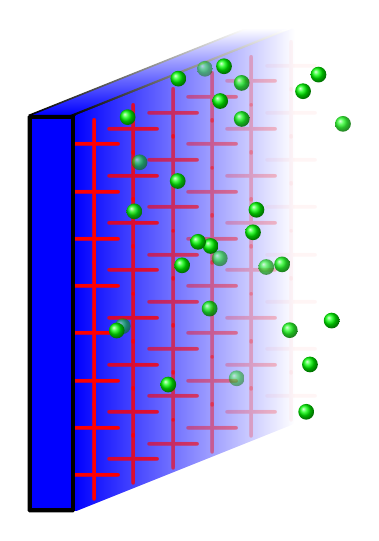
\begin{tikzpicture}[x=1cm, y=1cm]
\begin{scope}[every node/.append style={
	yslant=0,xslant=0},yslant=0,xslant=2.5
]
\shade[bottom color = black, top color = white] (-12.54, 5)
rectangle +(0.1, 1.1);
\shade[bottom color = blue, top color = white] (-12.48,5)
rectangle +(0.5,1.1);
\shade[bottom color = black, top color = white] (-12, 4.98)
rectangle +(0.1, 1.1);
\end{scope}

\begin{scope}[every node/.append style={
	yslant=0,xslant=0},yslant=0.4,xslant=0
]
\shade[left color = blue, right color = white, rounded corners=1]
(0.54,-0.26) rectangle +(2.8,5.03);
\foreach \x in {0.8,1.3,...,3.3}{
	\foreach \y in {0.1, 0.7,..., 4.8}{
		\pgfmathsetmacro{\val}{1-(\x-0.8)/2.6}
		\node [color = red, opacity =\val] at (\x ,\y) {\Huge{\textbf +}};
	}
}
\end{scope}

\pgfmathsetseed{10}

\foreach \i in {1,2,...,30}{
	%    \pgfmathsetmacro{\x}{(rand*0.5 + 1)*4 + 1}
	%    \pgfmathsetmacro{\y}{(rand*0.5 + 1)*3.9 + 2 }
	\pgfmathsetmacro{\x}{(rand*0.5 + 1)*3 - 0.5}
	\pgfmathsetmacro{\y}{(rand*0.5 + 1)*4.7-1.2}
	%    \pgfmathsetmacro{\opacVal}{0.95*(\x-2.5)/4 + rand*0.05}
	\pgfmathsetmacro{\opacVal}{rand*0.5+1}
	\shade [ball color = green, opacity = \opacVal] (\x,\y) circle (0.1);
}

\fill [fill = black,rounded corners= 0.6] (-0.05,-0.05)
rectangle +(0.6,5.05);
\fill [fill = blue] (0,0) rectangle +(0.5,4.95);
\end{tikzpicture}
	
\end{center}

\section{ví dụ 8 - câu lệnh vẽ tải trọng}

% Vector Styles
\tikzstyle{load}   = [ultra thick,-latex]
\tikzstyle{stress} = [-latex]
\tikzstyle{dim}    = [latex-latex]
\tikzstyle{axis}   = [-latex,black!55]

% Drawing Views
\tikzstyle{isometric}=[x={(0.710cm,-0.410cm)},y={(0cm,0.820cm)},z={(-0.710cm,-0.410cm)}]
\tikzstyle{dimetric} =[x={(0.935cm,-0.118cm)},y={(0cm,0.943cm)},z={(-0.354cm,-0.312cm)}]
\tikzstyle{dimetric2}=[x={(0.935cm,-0.118cm)},z={(0cm,0.943cm)},y={(+0.354cm,+0.312cm)}]
\tikzstyle{trimetric}=[x={(0.926cm,-0.207cm)},y={(0cm,0.837cm)},z={(-0.378cm,-0.507cm)}]

	\begin{center}
		\begin{tikzpicture}
		\node (origin) at (0,0) {}; % shift relative baseline
		\coordinate (O) at (2,3);
		\draw[fill=gray!10] (O) circle (1);
		\draw[fill=white] (O) circle (0.75) node[below,yshift=-1.125cm] {Mặt cắt};
		\draw[dim] (O) ++(-0.75,0) -- ++(1.5,0) node[midway,above] {$d_i$};
		\draw[dim] (O) ++(-1,1.25) -- ++(2,0) node[midway,above] {$d_o$}; 
		\foreach \x in {-1,1} {
			\draw (O) ++(\x,0.25) -- ++(0,1.25);
		}
		\end{tikzpicture}%
		\begin{tikzpicture}[dimetric2]
		\coordinate (O) at (0,0,0);
		\draw[axis] (O) -- ++(6,0,0) node[right] {$x$};
		\draw[axis] (O) -- ++(0,6,0) node[above right] {$y$};
		\draw[axis] (O) -- ++(0,0,6) node[above] {$z$};
		\draw[fill=gray!50] (0,0,-0.5) circle (0.5); 
		\fill[fill=gray!50] (-0.46,-0.2,-0.5) -- (0.46,0.2,-0.5) -- (0.46,0.2,0) -- (-0.46,-0.2,0) -- cycle;
		\draw[fill=gray!20] (O) circle (0.5);
		\draw (0.46,0.2,-0.5) -- ++(0,0,0.5) node[below right,pos=0.0] {Giá đỡ cố định};
		\draw (-0.46,-0.2,-0.5) -- ++(0,0,0.5);
		\draw[fill=gray!10] (O) circle (0.2);
		\fill[fill=gray!10] (-0.175,-0.1,0) -- (0.175,0.1,0) -- ++(0,0,4) -- (-0.175,-0.1,4) -- cycle;
		\draw (-0.175,-0.1,0) -- ++(0,0,4);
		\draw (0.175,0.1,0) -- ++(0,0,4) node[right,midway] {Thép};
		\draw (4,0,3.95) -- ++(0,0,-1);
		\foreach \z in {0.5,0.75,...,5} {
			\draw[-latex] (-2*\z/5-0.2,0,\z) -- (-0.2,0,\z);
		}
		\draw[load] (0,0,4) -- ++(0,0,-1.25) node[right,xshift=0.1cm] {$F_{z1}$};
		\draw[fill=gray!20] (-0.25,-0.25,5) -- (4,-0.25,5) -- (4,+0.25,5) -- (-0.25,+0.25,5) -- cycle; 
		\draw[fill=gray!50] (+4.00,-0.25,4) -- (4,+0.25,4) -- (4,+0.25,5) -- (+4.00,-0.25,5) -- cycle; 
		\draw[fill=gray!10] (-0.25,-0.25,4) -- (4,-0.25,4) -- (4,-0.25,5) -- (-0.25,-0.25,5) -- cycle; 
		\draw (4.05,0,4) -- ++(1,0,0);
		\draw (4.05,0,5) -- ++(1,0,0);
		\draw[dim] (4.5,0,0) -- ++(0,0,4) node[midway,right] {$h_1$};
		\draw[dim] (4.5,0,4) -- ++(0,0,1) node[midway,right] {$h_2$};
		\draw[dim] (0,0,3.4) -- ++(4,0,0) node[midway,below] {$b_2$};
		\coordinate (P) at (2,-0.25,4.5);
		\draw (P) -- ++(0,0,0.25);
		\draw (P) -- ++(0.25,0,0);
		\draw[dim] (2.125,-0.25,4.5) -- ++(0,0,-0.5) node[midway,right] {$z_1$};
		\draw[dim] (2,-0.25,4.625) -- ++(-2,0,0) node[midway,below] {$x_1$};
		\draw[load] (2,-2.45,4.5) -- ++(0,2.2,0) node[pos=0.0,right,xshift=0.08cm] {$F_{y1}$};
		\draw[axis,dashed,-] (O) -- (0,0,5);
		\draw (0,0,5.5) -- ++(4,0,0) node[midway,above] {$w_{z}$};
		\foreach \x in {0,0.25,...,4} {
			\draw[-latex] (\x,0,5.5) -- ++(0,0,-0.5);
		}
		\draw (-0.2,0,0) -- ++(-2,0,5) node[above,xshift=0.5cm] {$w_{x}=\frac{z}{h_1+h_2} w_0$};
		\end{tikzpicture} %
	\end{center}

\section{Ví dụ 9 - vẽ biểu đồ thời gian}

\newcounter{wavenum}

\setlength{\unitlength}{1cm}
% advance clock one cycle, not to be called directly
\newcommand*{\clki}{
	\draw (t_cur) -- ++(0,.3) -- ++(.5,0) -- ++(0,-.6) -- ++(.5,0) -- ++(0,.3)
	node[time] (t_cur) {};
}

\newcommand*{\bitvector}[3]{
	\draw[fill=#3] (t_cur) -- ++( .1, .3) -- ++(#2-.2,0) -- ++(.1, -.3)
	-- ++(-.1,-.3) -- ++(.2-#2,0) -- cycle;
	\path (t_cur) -- node[anchor=mid] {#1} ++(#2,0) node[time] (t_cur) {};
}

% \known{val}{length}
\newcommand*{\known}[2]{
	\bitvector{#1}{#2}{white}
}

% \unknown{length}
\newcommand*{\unknown}[2][XXX]{
	\bitvector{#1}{#2}{black!20}
}

% \bit{1 or 0}{length}
\newcommand*{\bit}[2]{
	\draw (t_cur) -- ++(0,.6*#1-.3) -- ++(#2,0) -- ++(0,.3-.6*#1)
	node[time] (t_cur) {};
}

% \unknownbit{length}
\newcommand*{\unknownbit}[1]{
	\draw[ultra thick,black!50] (t_cur) -- ++(#1,0) node[time] (t_cur) {};
}

% \nextwave{name}
\newcommand{\nextwave}[1]{
	\path (0,\value{wavenum}) node[left] {#1} node[time] (t_cur) {};
	\addtocounter{wavenum}{-1}
}

% \clk{name}{period}
\newcommand{\clk}[2]{
	\nextwave{#1}
	\FPeval{\res}{(\wavewidth+1)/#2}
	\FPeval{\reshalf}{#2/2}
	\foreach \t in {1,2,...,\res}{
		\bit{\reshalf}{1}
		\bit{\reshalf}{0}
	}
}

% \begin{wave}[clkname]{num_waves}{clock_cycles}
\newenvironment{wave}[3][clk]{
	\begin{tikzpicture}[draw=black, yscale=.7,xscale=1]
	\tikzstyle{time}=[coordinate]
	\setlength{\unitlength}{1cm}
	\def\wavewidth{#3}
	\setcounter{wavenum}{0}
	\nextwave{#1}
	\foreach \t in {0,1,...,\wavewidth}{
		\draw[dotted] (t_cur) +(0,.5) node[above] {t=\t} -- ++(0,.4-#2);
		\clki
	}
}{\end{tikzpicture}}

%%% End of timing.sty

	\begin{wave}{13}{5}
		\nextwave{req\_addr} \bit{0}{.2} \bit{1}{1} \bit{0}{3} \bit{1}{1} \bit{0}{.8}
		\nextwave{inst\_addr} \unknown[X]{.5} \known{addr}{1} \unknown{4.5}
		\nextwave{link\_addrs} \unknown{1.2} \known{map}{1} \unknown{3.8}
		\nextwave{link\_load} \unknown{2.2} \known{vam}{1} \unknown{2.8}
		\nextwave{link\_load\_r} \unknown{3.1} \known{val}{1} \unknown{1.9}
		\nextwave{simulate} \bit{0}{3.1} \bit{1}{1} \bit{0}{1.9}
		\nextwave{output} \unknown{3.3} \known{}{.5} \known{}{.5} \unknown{1.7}
		\nextwave{prev\_output} \unknown{3.2} \known{old}{1} \unknown{1.8}
		\nextwave{differs} \unknownbit{3.3} \bit{1}{.5} \bit{1}{.4} \unknownbit{1.8}
		\nextwave{differs\_r} \unknownbit{4.1} \bit{1}{1} \unknownbit{.9}
		\nextwave{dep\_addr} \unknown{4.2} \known{dep}{1} \unknown[X]{.8}
		\nextwave{req} \unknown{4.3} \known{req}{1} \unknown[X]{.7}
	\end{wave}
	%%% có thể thay đổi

\end{document}
